\documentclass[11pt]{article}

\usepackage[margin=0.75in]{geometry}
\usepackage{url}
\usepackage{graphicx}
\usepackage{float}
\graphicspath{ {figs/} }

\title{An Analysis of fcMRI data in Schizophrenia}
\author{
  Hejazi, Nima\\
  \texttt{nhejazi}
  \and
  Lin, Feng\\
  \texttt{LiamFengLin}
  \and
  Zhao, Luyun\\
  \texttt{lynnzhao92}
  \and
  Zhou, Xinyue\\
  \texttt{z357412526}
}

\bibliographystyle{siam}

\begin{document}
\maketitle

\abstract{We report analyses intended to explore the functional magnetic
  resonance imaging (fMRI) data collected in studies conducted by Repovs et al.,
on the manner in which brain network connectivity is related to schizophrenia
\cite{repovs2011,repovs2012}. A host of exploratory analyses, combining both
classical linear modeling methods and machine learning, were used in order
to gain further insights into the fMRI data examined.}

\section{Introduction}

The human central nervous system is a complex dynamic network, consisting of
numerous functional regions that coordinate everything from simple reflexes to
complicated thoughts. In an effort to better understand the manner in which
functional changes contribute to the symptoms of schizophrenia, Repovs \textit{et
al.} conducted neuroimaging studies, including both functional connectivity
magnetic resonance imaging (fcMRI) and diffusion tensor imaging (DTI), on many
subjects, with their goal being to characterize the activity of several brain
regions chosen \textit{a priori}, and to develop an understanding of how the functional 
activities of these regions may differ across health states \cite{repovs2011,repovs2012}.

\subsection{Generalized Linearl Model}

The goal of GLM with respect to our dataset is to detect the activation clusters of target and non-target events in one subject in the control (healthy) group. An activation cluster refers to a group of neighboring voxels activated beyond certain statistical threshold (t-test p value) by defined events. We did not set up a quantifiable criterion for example, to definitively separate one cluster from a neighboring cluster, but provide qualitative evidence in terms of beta and p values map. The target and non-target events are defined in the method section below. 

Additionally, GLM is performed for both 0-back and 2-back tasks for the subject so that we can assess the effect of different memory load on activation clusters. Also, through the GLM, we can access the noise structure of the data so that we can remove the noise regressors in connectivity analysis.

Besides analysis pertaining to our goals, we performed various exploratory data analysis (EDA) such as k-means, correlations with different baseline functions that helped in understanding the data. The details of EDA and discussion of the results are in the appendix. 

\subsection{Connectivity Analysis}

We are interested in the response of the brain of the schizophrenia patients in a memory-related task, compared to the healthy controls. The goal of connectivity analysis is to compare the functional brain connectivity, measured by ROI-ROI correlations of 2-back task data between the four networks of the brain (DMN,FP,CO,CER), across CON and SCZ groups. CON is defined as the control group and their siblings and SCZ is defined as the schizophrenia individuals and their siblings. The task data was preprecessed by removing the noise regressors after fitting the GLM described above. The four networks are thought to be critical for cognitive function and as defined in the paper (paper 1): (1) a default mode network (DMN); (2) a dorsal fronto-parietal network (FP); (3) a cingula-opercular network (CO); (4) a cerebellar network (CER). We choose to focus on 2-back task because it is the most difficult to perfom among the three levels of n-back tasks and requires the highest memory load, thus more likely to reveal the difference of the response of the brain of the patients and the controls. 

\section{Data}

The analyses reported in this paper are based on data generated in a series of
neuroimaging experiments conducted by Barch, Repovs, \& Csernansky. The aim of
these experiments was to ascertain the activity of several brain networks
thought to be associated with depressed cognitive function in individuals with
schizophrenia by collecting functional connectivity magnetic resonance imaging
(fcMRI) data on healthy individuals, individuals with schizophrenia, and the
(healthy) siblings of participants in either of the two former groups
\cite{repovs2012}. For the purposes of the analyses reported in this paper, the imaging
data were acquired from the OpenfMRI project (\url{https://openfmri.org/}), where they
are listed with accession number ds115. The data is available for groups of
subjects, with each subject-specific data directory containing anatomical MR
imaging data, functional MR imaging (using the BOLD contrast) data, and
diffusion tensor imaging (DTI) data. In this preliminary report, the analyses
are restricted to the BOLD functional MR imaging data, for 8 subjects among
the pool of 102 subjects for which data are available, with most analyses
(ranging from linear modeling to machine learning with K-Means) taking the form
of exploratory examinations into the structure of this imaging data.


\section{Methods}

\subsection{Data Preprocessing}

For all BOLD datasets used in analysis, we removed the first five images to allow measurements to achieve steady state. They were preprocessed with 1. motion correction (coregistration in time to partially correct for movement during the run and between runs)
2. temporary high-pass filtering to remove low frequency drifts / noise; 3. registration to a standard anatomical template (the MNI template). Additionally, each image was passed thorugh a gaussian filter of sigma=2. This spatial smoothing approach assumes that fMRI data inherently show spatial correlations due to functional similarities of adjacent brain regions. To address the fact that boundary voxels of the brain are smoothed with meansurements outside the brain, we implemented substitution of voxels near but outside the boundaries of brain with neighboring measurements within the boundary of the brain.
However, the current analysis was performed without padding because the implementation was very slow.

\subsection{Data Analysis}

\subsubsection{Generalized Linear Model}

Before the discussion on the specifics of our GLM, it is worthwhile to discuss
the details of the condition files in the dataset because we make use of all
condition files in the GLM. The keys in Metadata folder of the dataset does not
correpsond to the condition files so the keys and the related descriptions of
the condition files are redefined as below. 

\begin{itemize}

\item cond001: Start cues for both blocks of the run.

\item cond002: The visual stimuli (i.e. letters) presenteed to the subject. The
intensities are all one becasue there is only one homogeneous event type.

\item cond003: The target and non-target events during the run. A target is the event
that the current letter that is the same as the nth preceeding letter. Note that
for 0-back, the 0th preceeding letter is pre-specificed before the run instead
of being presented continuously throughout the run. A non-target is the opposite
of a target, in which the current letter is not the same. 

\item cond004: Done cues for both blocks of the run.

\item cond005: Start and durations of the two blocks with a rest (i.e. fixation)
period in between the blocks. This is different from resting-state data, which
is mentioned in the reference papers but is not included on the OpenfMRI
website. 

\item cond006: This is unknown and is not explained in the paper.

\item cond007: Errors made by the subject when responding for each letter shown
whether it was the same as a pre-specified (0-back) or preceding (1,2-back)
letter.

\end{itemize}

We can now turn to describe the regressors in the GLM on each voxel time
course. For all convolutions below, we convolve a specified condition file
on-off time course at a time unit of 0.01 TR with a gamma function and take the
convolved values at the start of each TR.

\begin{itemize}
\item reg001: Convolution of target events from cond003. Essentially, we split cond003
into separate regressors, target and non-target with the assumption that they
different in the levels of activitities.

\item reg002: Convolution of non-target events from cond003.

\item reg003: On-off time course from cond005. This regressor is included to account
for mean differences in the two blocks of the same run.

\item reg004: Convolution of start cues from cond001. This is separated from the
target and non-target regressors in that it is not part of tasks and that it is
not likely to involve heavy working memory load as tasks.

\item reg005: Convolution of done cues from cond004. It has the same purpose as
reg004.

\item reg006 and reg007: A linear drift term and a quadratic drift term included as
potential nuisansance regressors. Their significance is investigated below.

\item reg007: A quadratic drift term includede as a potential nuisansance regressors. 

\item reg008 and reg009: The first two principal components of the data. Based on the
projections shown below, we decide that the first two are not functional
features.

\item reg010: Intercept term.

\end{itemize}

\begin{figure}
\centering
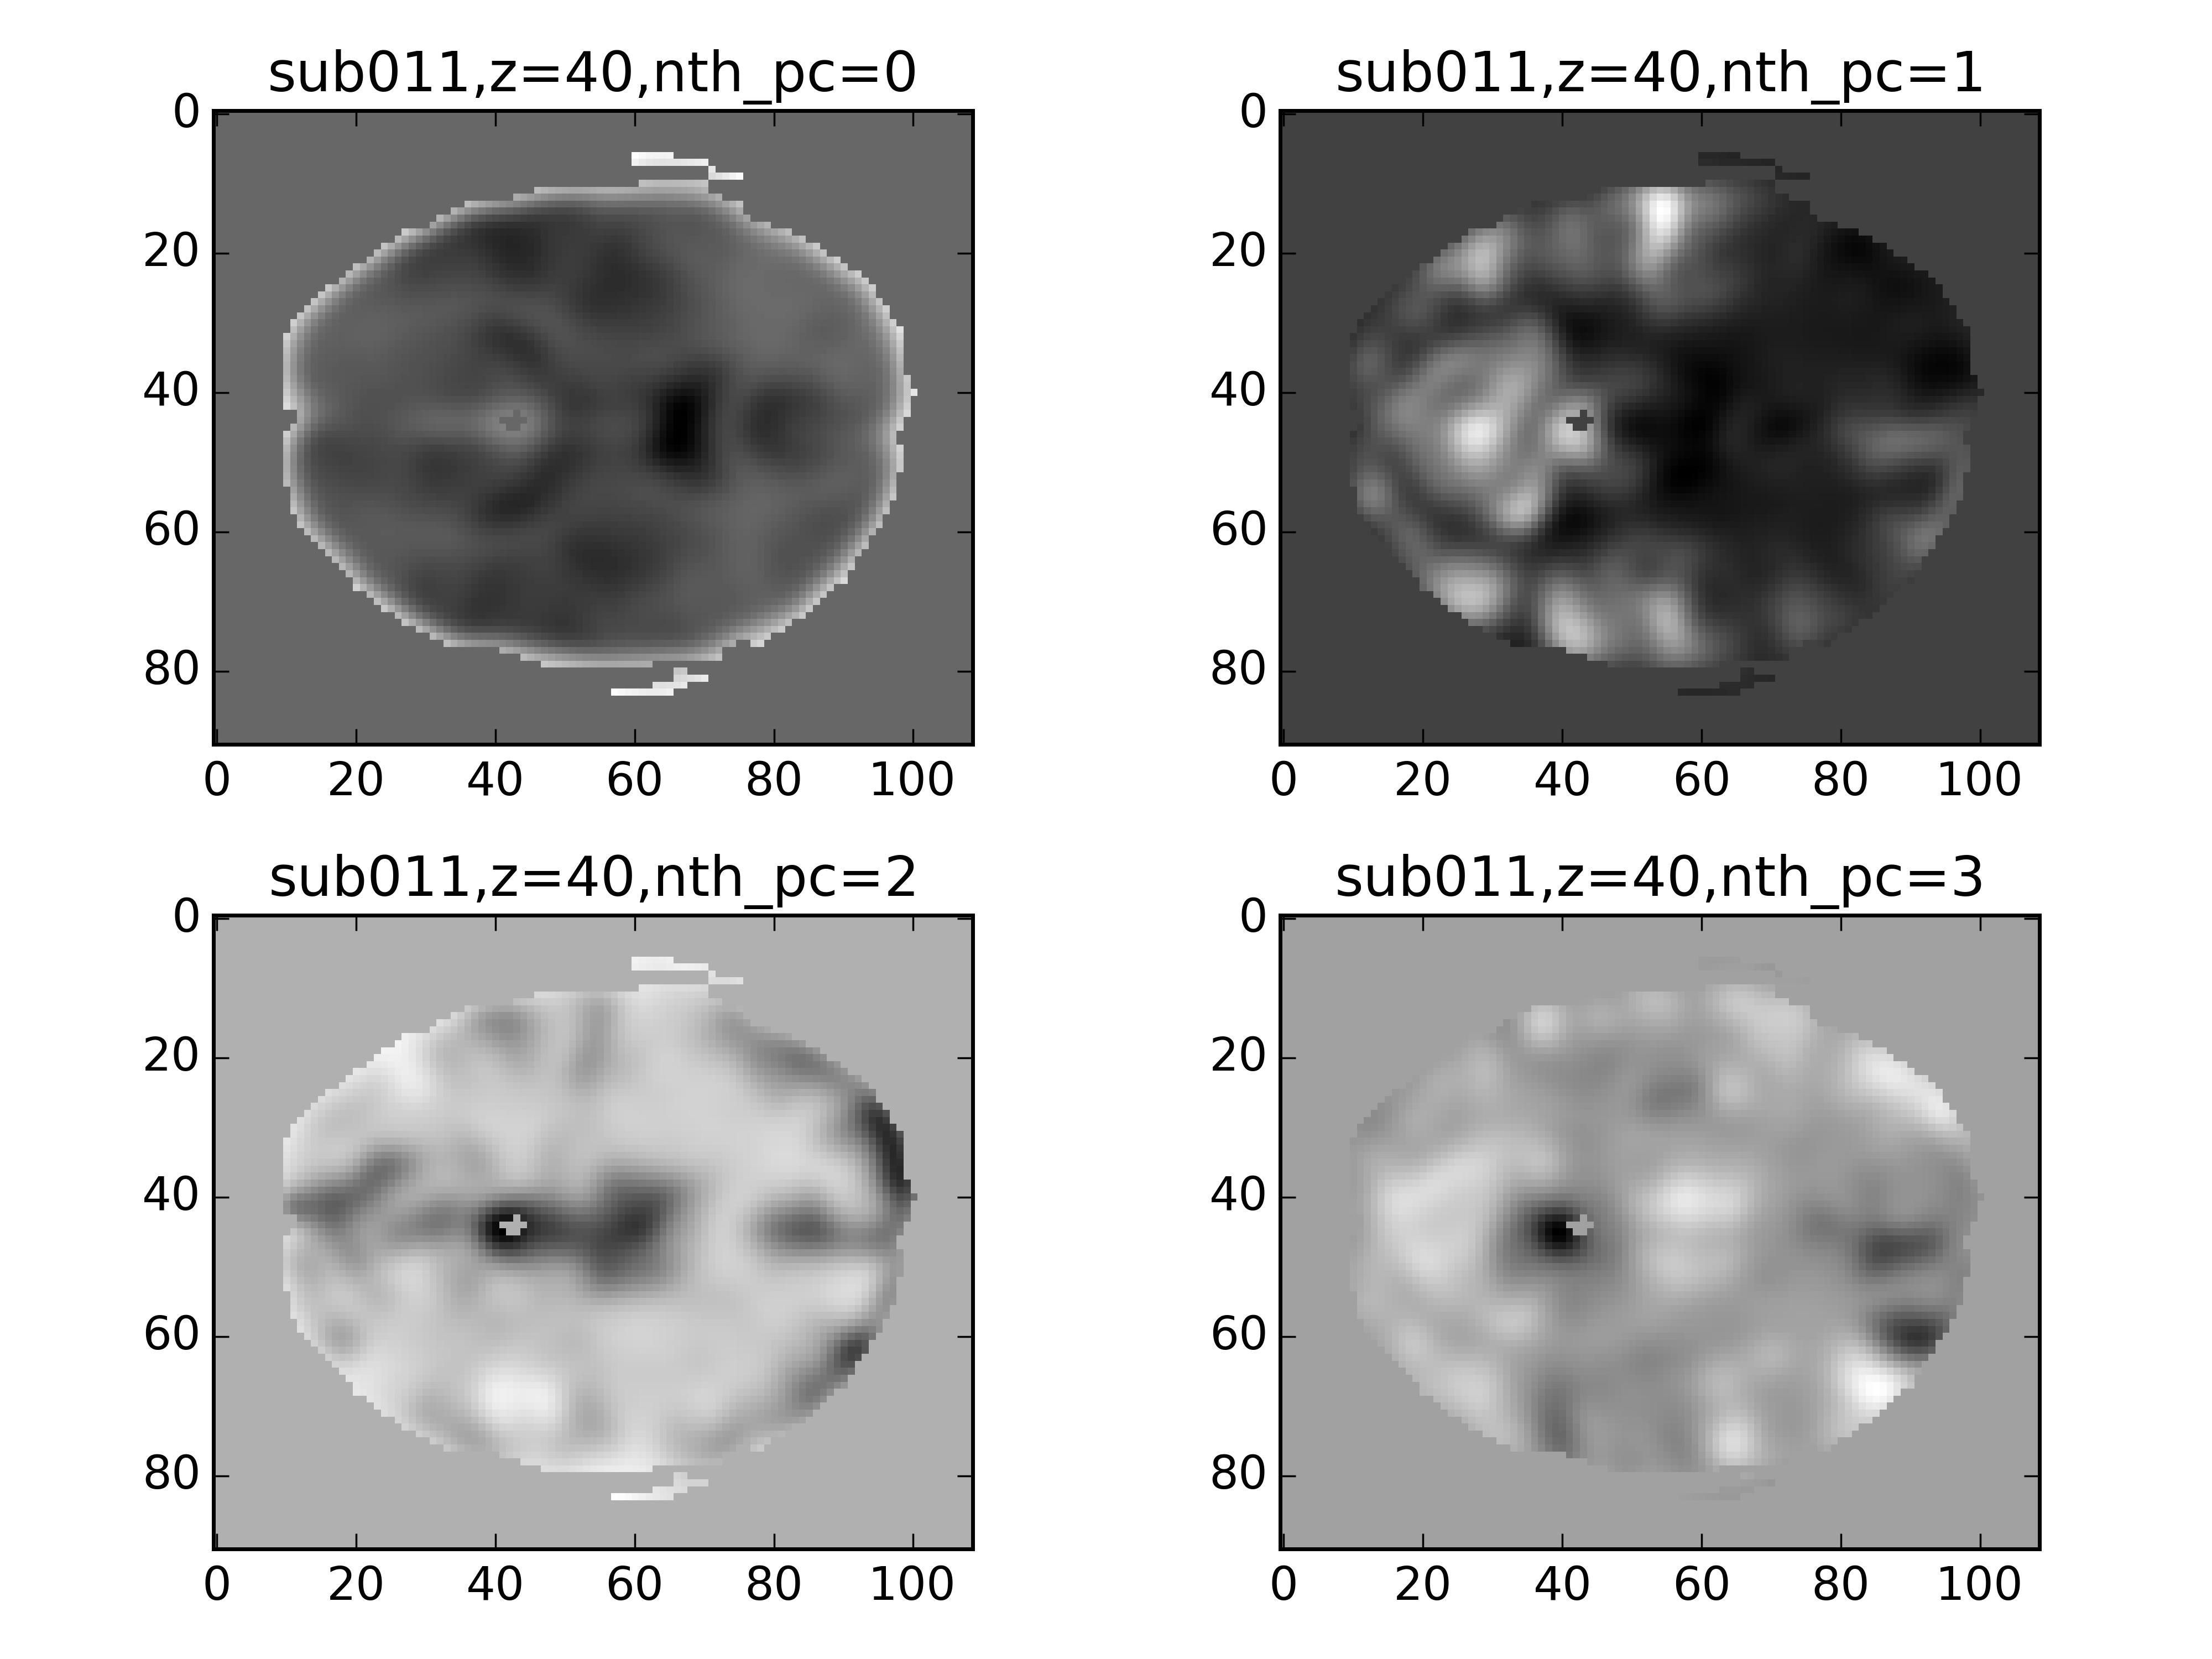
\includegraphics[scale=0.3]{figs/glm_graphs/sub011_task001_first_four_pcs.png}
\caption{The first four principal components for subject 011}
\end{figure}

For each $\beta$ on each voxel time course, a linear regression two-tailed
t-test is conducted to access whether there is a significant linear relationship
between the dependent variable Y and the regressor associated with the $\beta$
with significance levels of 0.05.

null hypothesis: $ \beta = 0$ 
alternative hypothesis: $\beta \neq 0$

Instead of plotting out the regions of siginifcant p-values, the p-value map of
the entire brain is presented as results. 

Before performing t-test, we access the validity of t-tests by examining its
assumptions. The two main assumptions are 1. the residuals of each linear model
are independent and identically distribued (i.i.d); 2. residuals for the model
are normally distributed. Shapiro-Wilk Test is performed on the residuals of
each voxel time course linear model. 37703 out of 207766 voxels fail the
test. However, when perform a large number of statistical tests, some will have
p values less than 0.05 purely by chance. To test the normality of several
models together, three multiple comparison tests, namely, Bonferroni,
Hochberg's and Benjamini-Hochberg, are performed and results are shows below:

Bonferroni: normality assumption is violated in 6 voxels.
Hochberg: normality assumption is violated in 262 voxels.
Benjamini-Hochberg: all of voxels pass the normality test.

In summary, we can conclude that our assumption of normality in residuals is
generally valid.

\subsubsection{Connectivity Analysis}

The roadmap for the analytic steps followed to examin connectivity is as
follows:

\begin{enumerate}
  \item Removal of noise regressors from the voxel time series. Linear model as
    defined in the GLM section was fitted to each of the BOLD dataset. The
    residuals after removal of the noise regressors (i.e. reg003 to reg010
    listed in the GLM section).
  \item Extraction of voxels per region of interst (ROI): ROIs of the four
    networks respectively are defined by a center and a diameter as 15mm (The
    reference paper ��). Two validations are made before the analysis: (1)
    it is ensured that the ROIs are non-overlapping by setting the diameters for
    each ROI sphere as less than the minimum distance between any two given ROIs
    in the full set, and (2) ROIs are represented as spheres instead of cubes in
    order to better approximate the underlying neurobiology and to easen the
    trouble associated with computing minimum distances between the ROIs in the
    set.
  \item In order to compute the ROI-ROI correlation, several steps were
    followed: (1) for each ROI in a given network, the corresponding voxels were
    extracted and their time series averaged to obtain a single average time
    series, (2) the ROI-ROI correlation is computed using the average time
    series, (3) for any two networks, which are composed with independent ROIs,
    we obtained the correlation matrix containing the correlation r-value of any
    two ROIs for the two networks, and (4) For each subject, we established the
    correlation matrix in (3) and group the r-values into two groups: CON and
    SCZ, according to the category of the subjects.  We decided to keep the
    original correlations to perform further analysis instead of 1) taking the
    mean of ROI-ROI r values per subject and 2) using Fisher's z
    transformation. Fisher's z transformation is a function of correlation r
    aimed at constructing a statistic asymptotically normal so that a variety of
    analysis and tests, such as computing confidence intervals, can be
    performed. Two requirements need to be met for z to be approximately normal:
    1) r is between variables from a bivariate normal distribution; 2) Sample
    size should be $n \geq 10$. Although some of the some samples shows a normal
    pattern based on normal Q-Q plot, many others have heavy-tailed density,
    violating the first requirement to arrive at a normal z value. Further more,
    in each ROI and network, more then 100 r's can be obtained, which means
    the distribution of r can be easily plotted. Also, abnormally high z values
    were present in our results because Fisher's z transformation has
    asymptotic behavior at r close to $ \pm 1$, causing the analysis to be
    extremely inaccurate had we chosen to z-transform the r values.
\end{enumerate}


\section{Results}

\subsection{Linear Modeling}

\begin{figure}
\centering
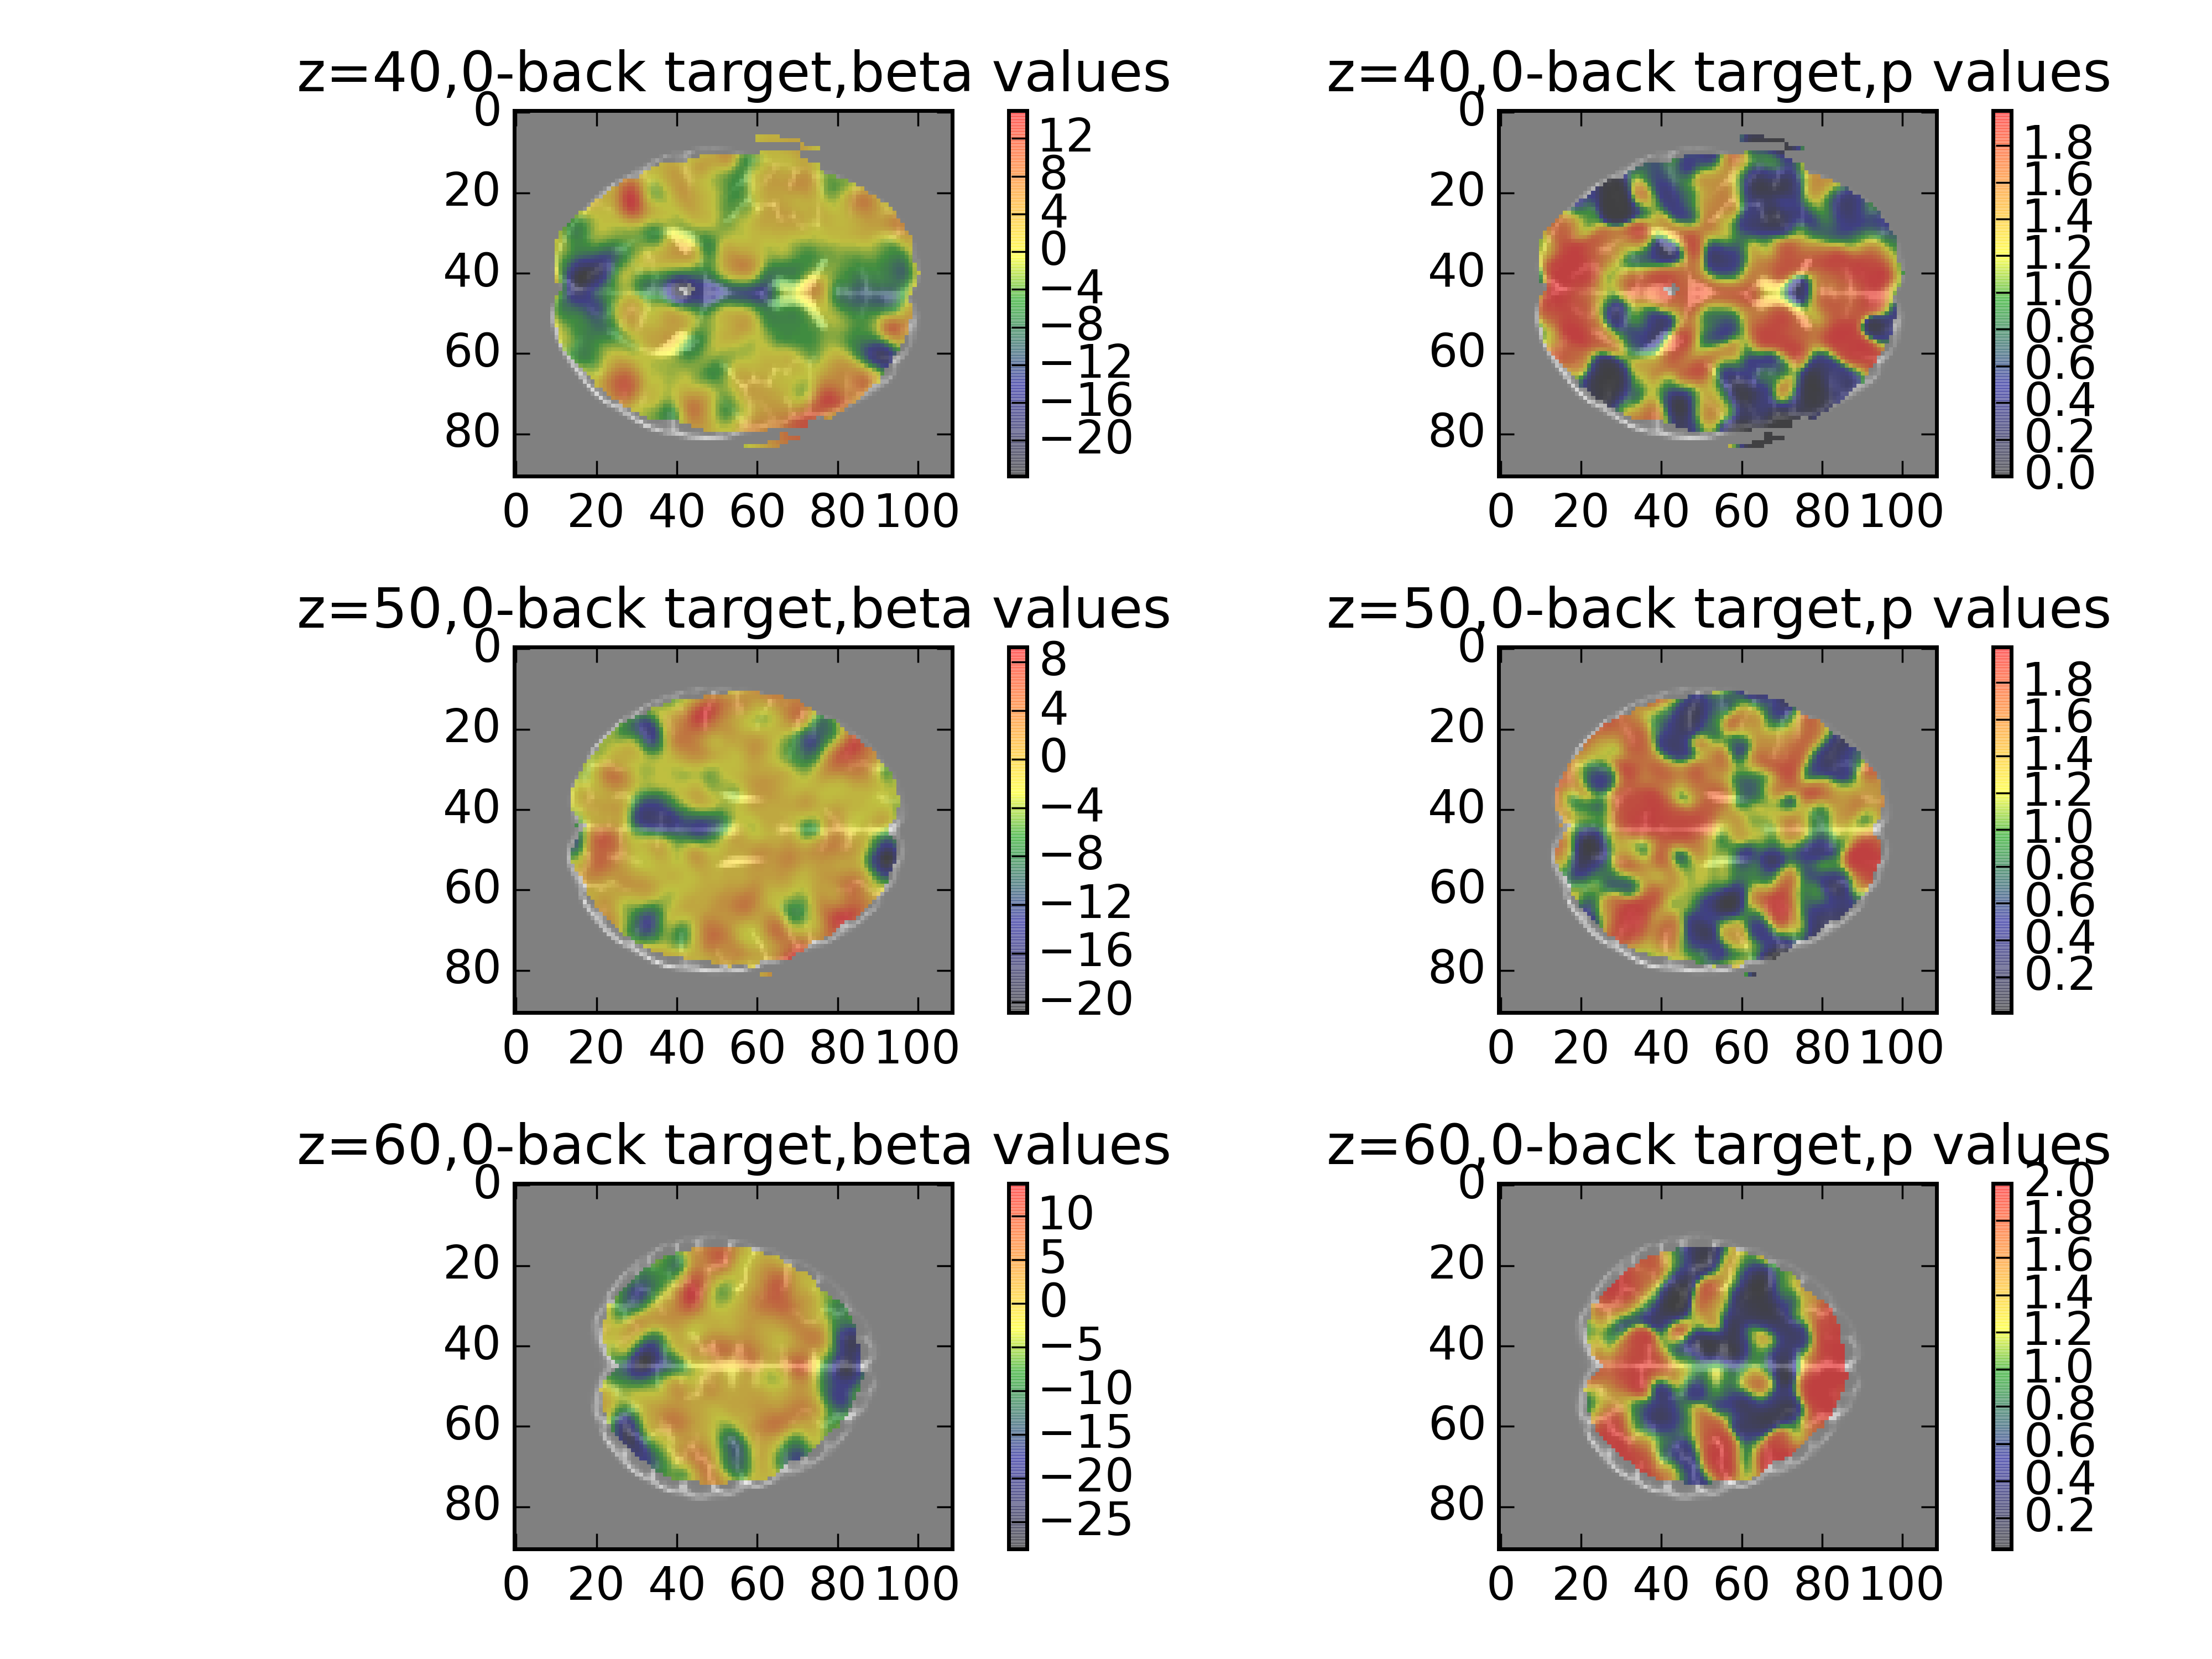
\includegraphics[scale=0.7]{figs/glm_graphs/sub011_target_betas_0_back.png}
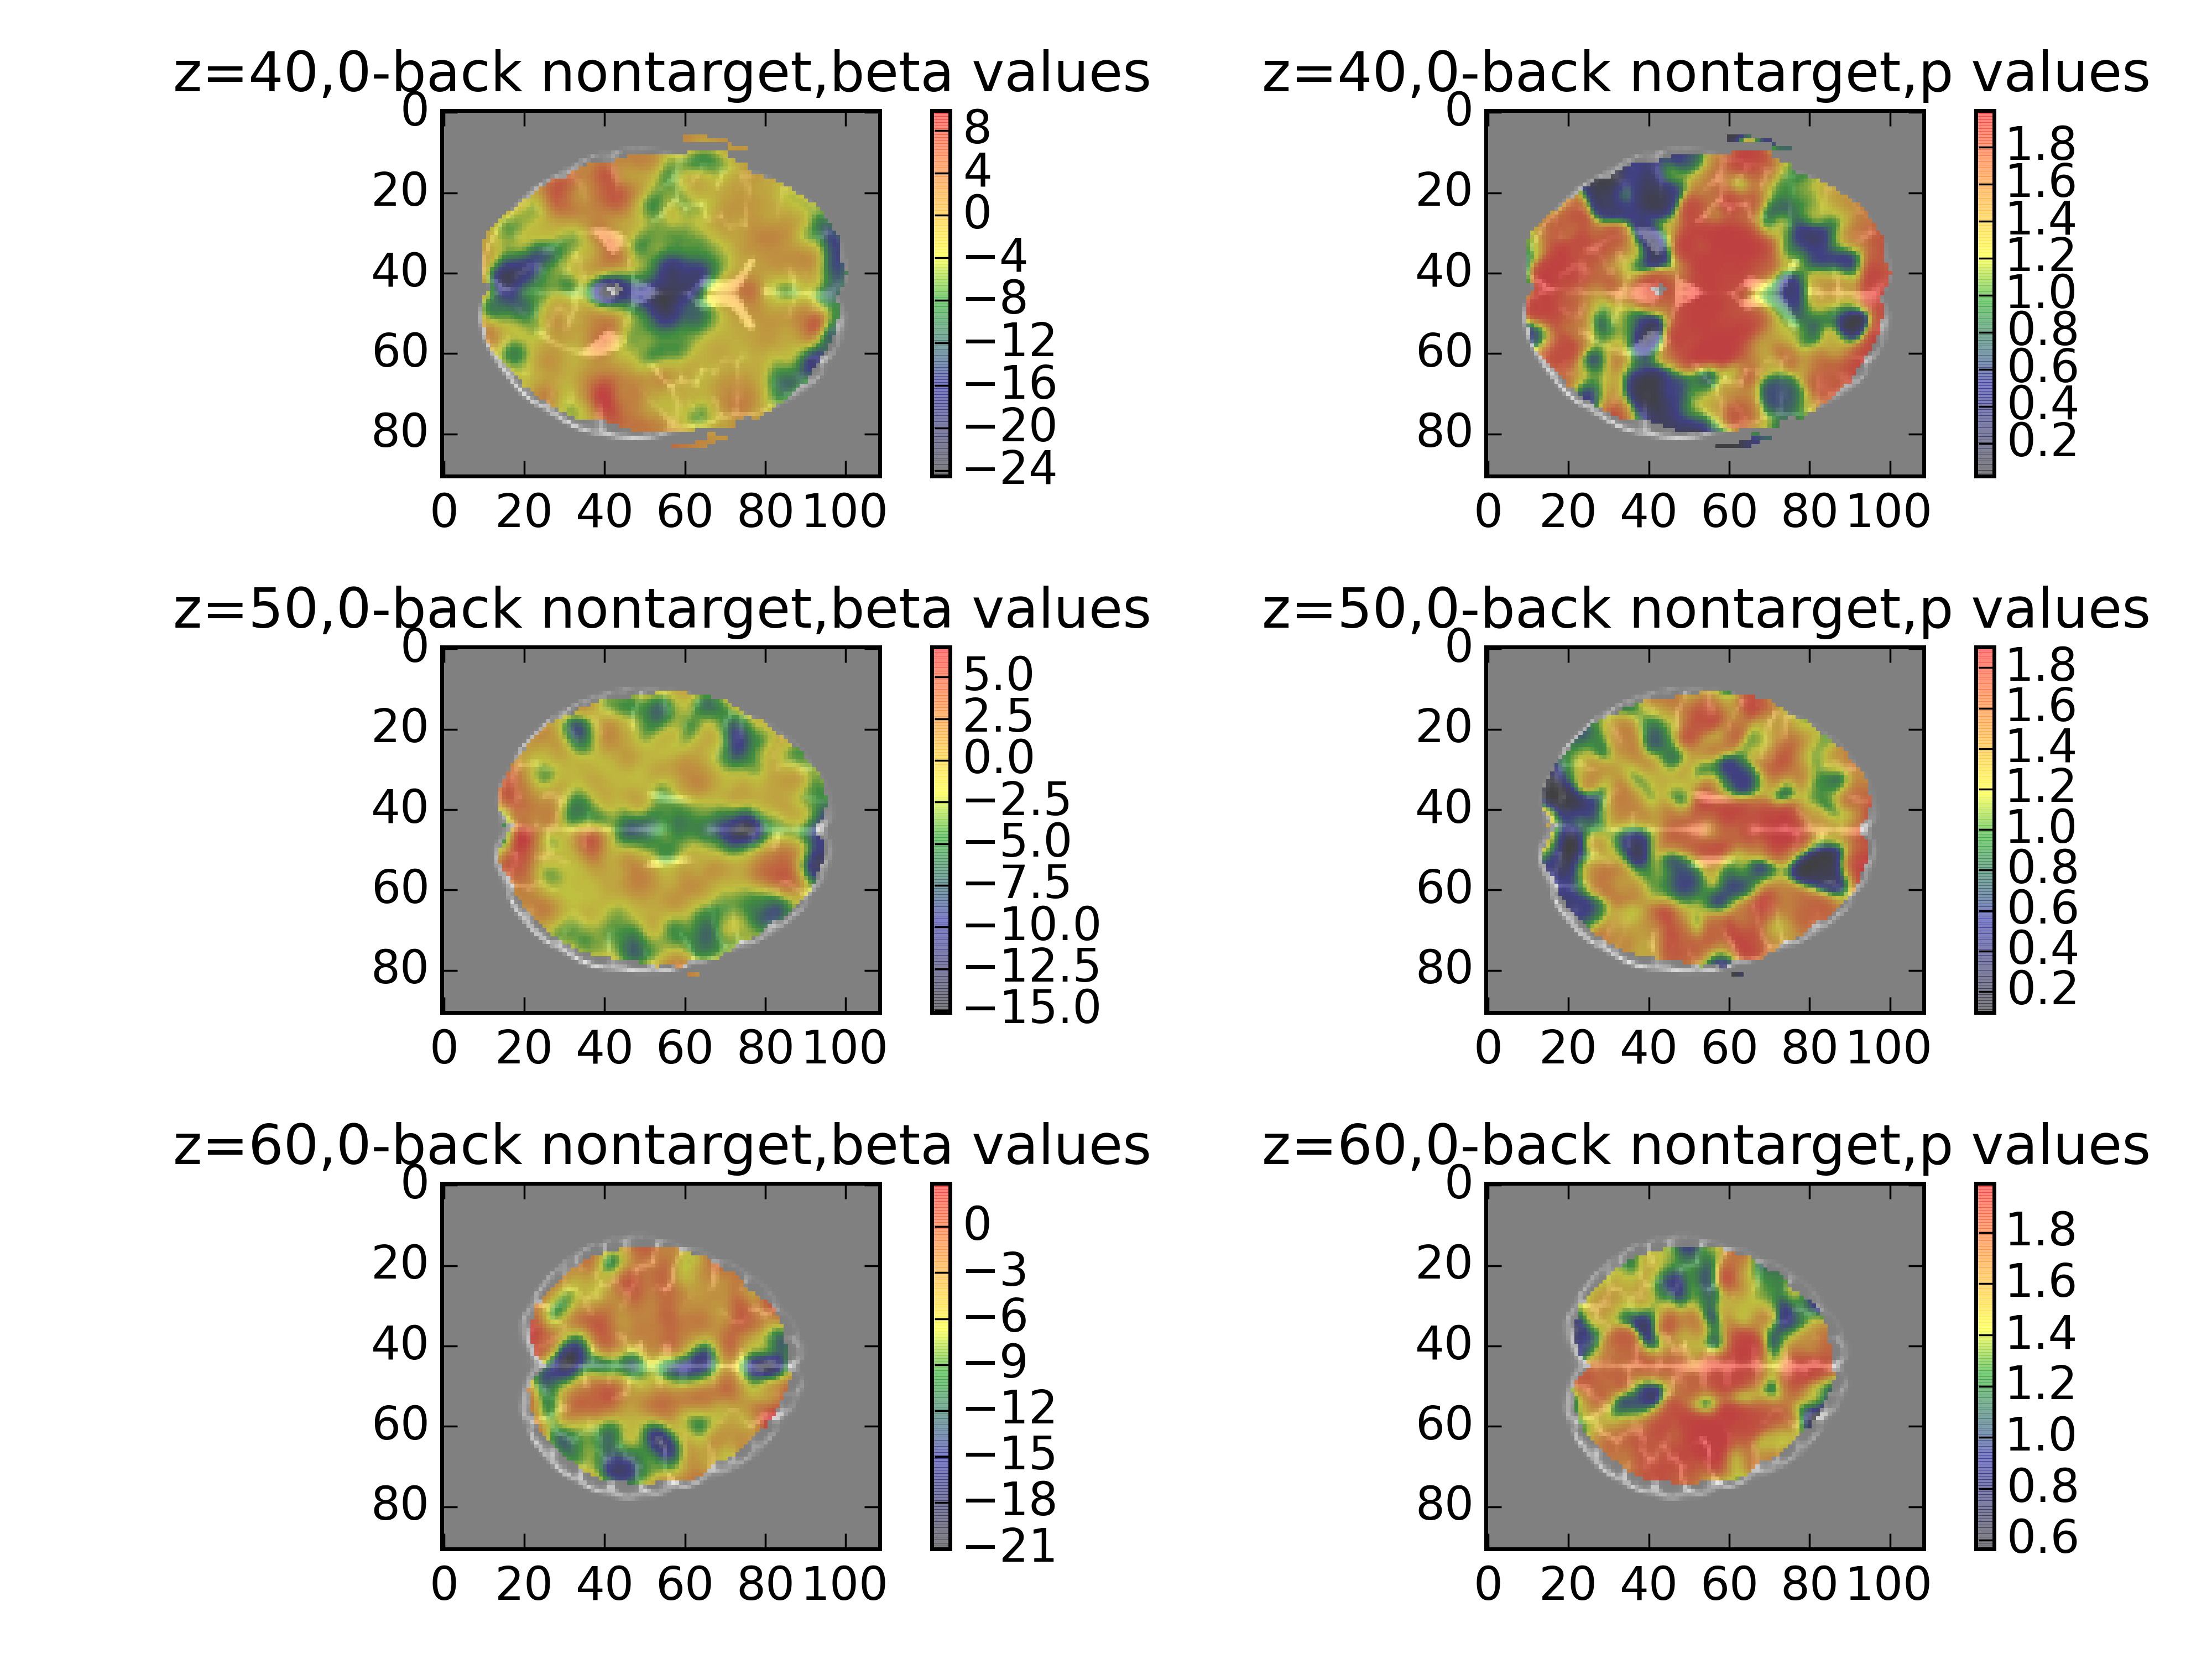
\includegraphics[scale=0.7]{figs/glm_graphs/sub011_nontarget_betas_0_back.png}
\caption{Above: 0-back target beta values and p values from two-tailed t tests against the null hypothesis of $\beta = 0$; Below: non-target beta values and p values from two-tailed t tests against the null hypothesis of $\beta = 0$}
\end{figure}

As the 0-back task serves primarily as an object recognition task with respect to the activation it induces in the central nervous system, it would be expected that visual processing centers of the brain would be found to be most activated. As seen in both the beta maps and the associated p-value maps, there is considerable (and significant) activation of occipital cortex as well as various regions of the frontal cortex. In contrast to the responses observed with respect to the 2-back task presented below, the coefficient maps for the 0-back task for target images indicates fair amounts of activity across many regions of the brain, as would be expected of a general recognition test, whereas, in the 2-back task for target images, there is noticeably increased magnitudes in the activation of regions in the occipital cortex and in the frontal lobes, as would be expected of a task that involves working memory. It is worth noting that there is considerably less difference between the 0-back target vs. nontarget activation patterns than between the 2-back target vs. nontarget activation patterns, agreeing with the expectations based on psychological constructs such as working memory.

\begin{figure}
\centering
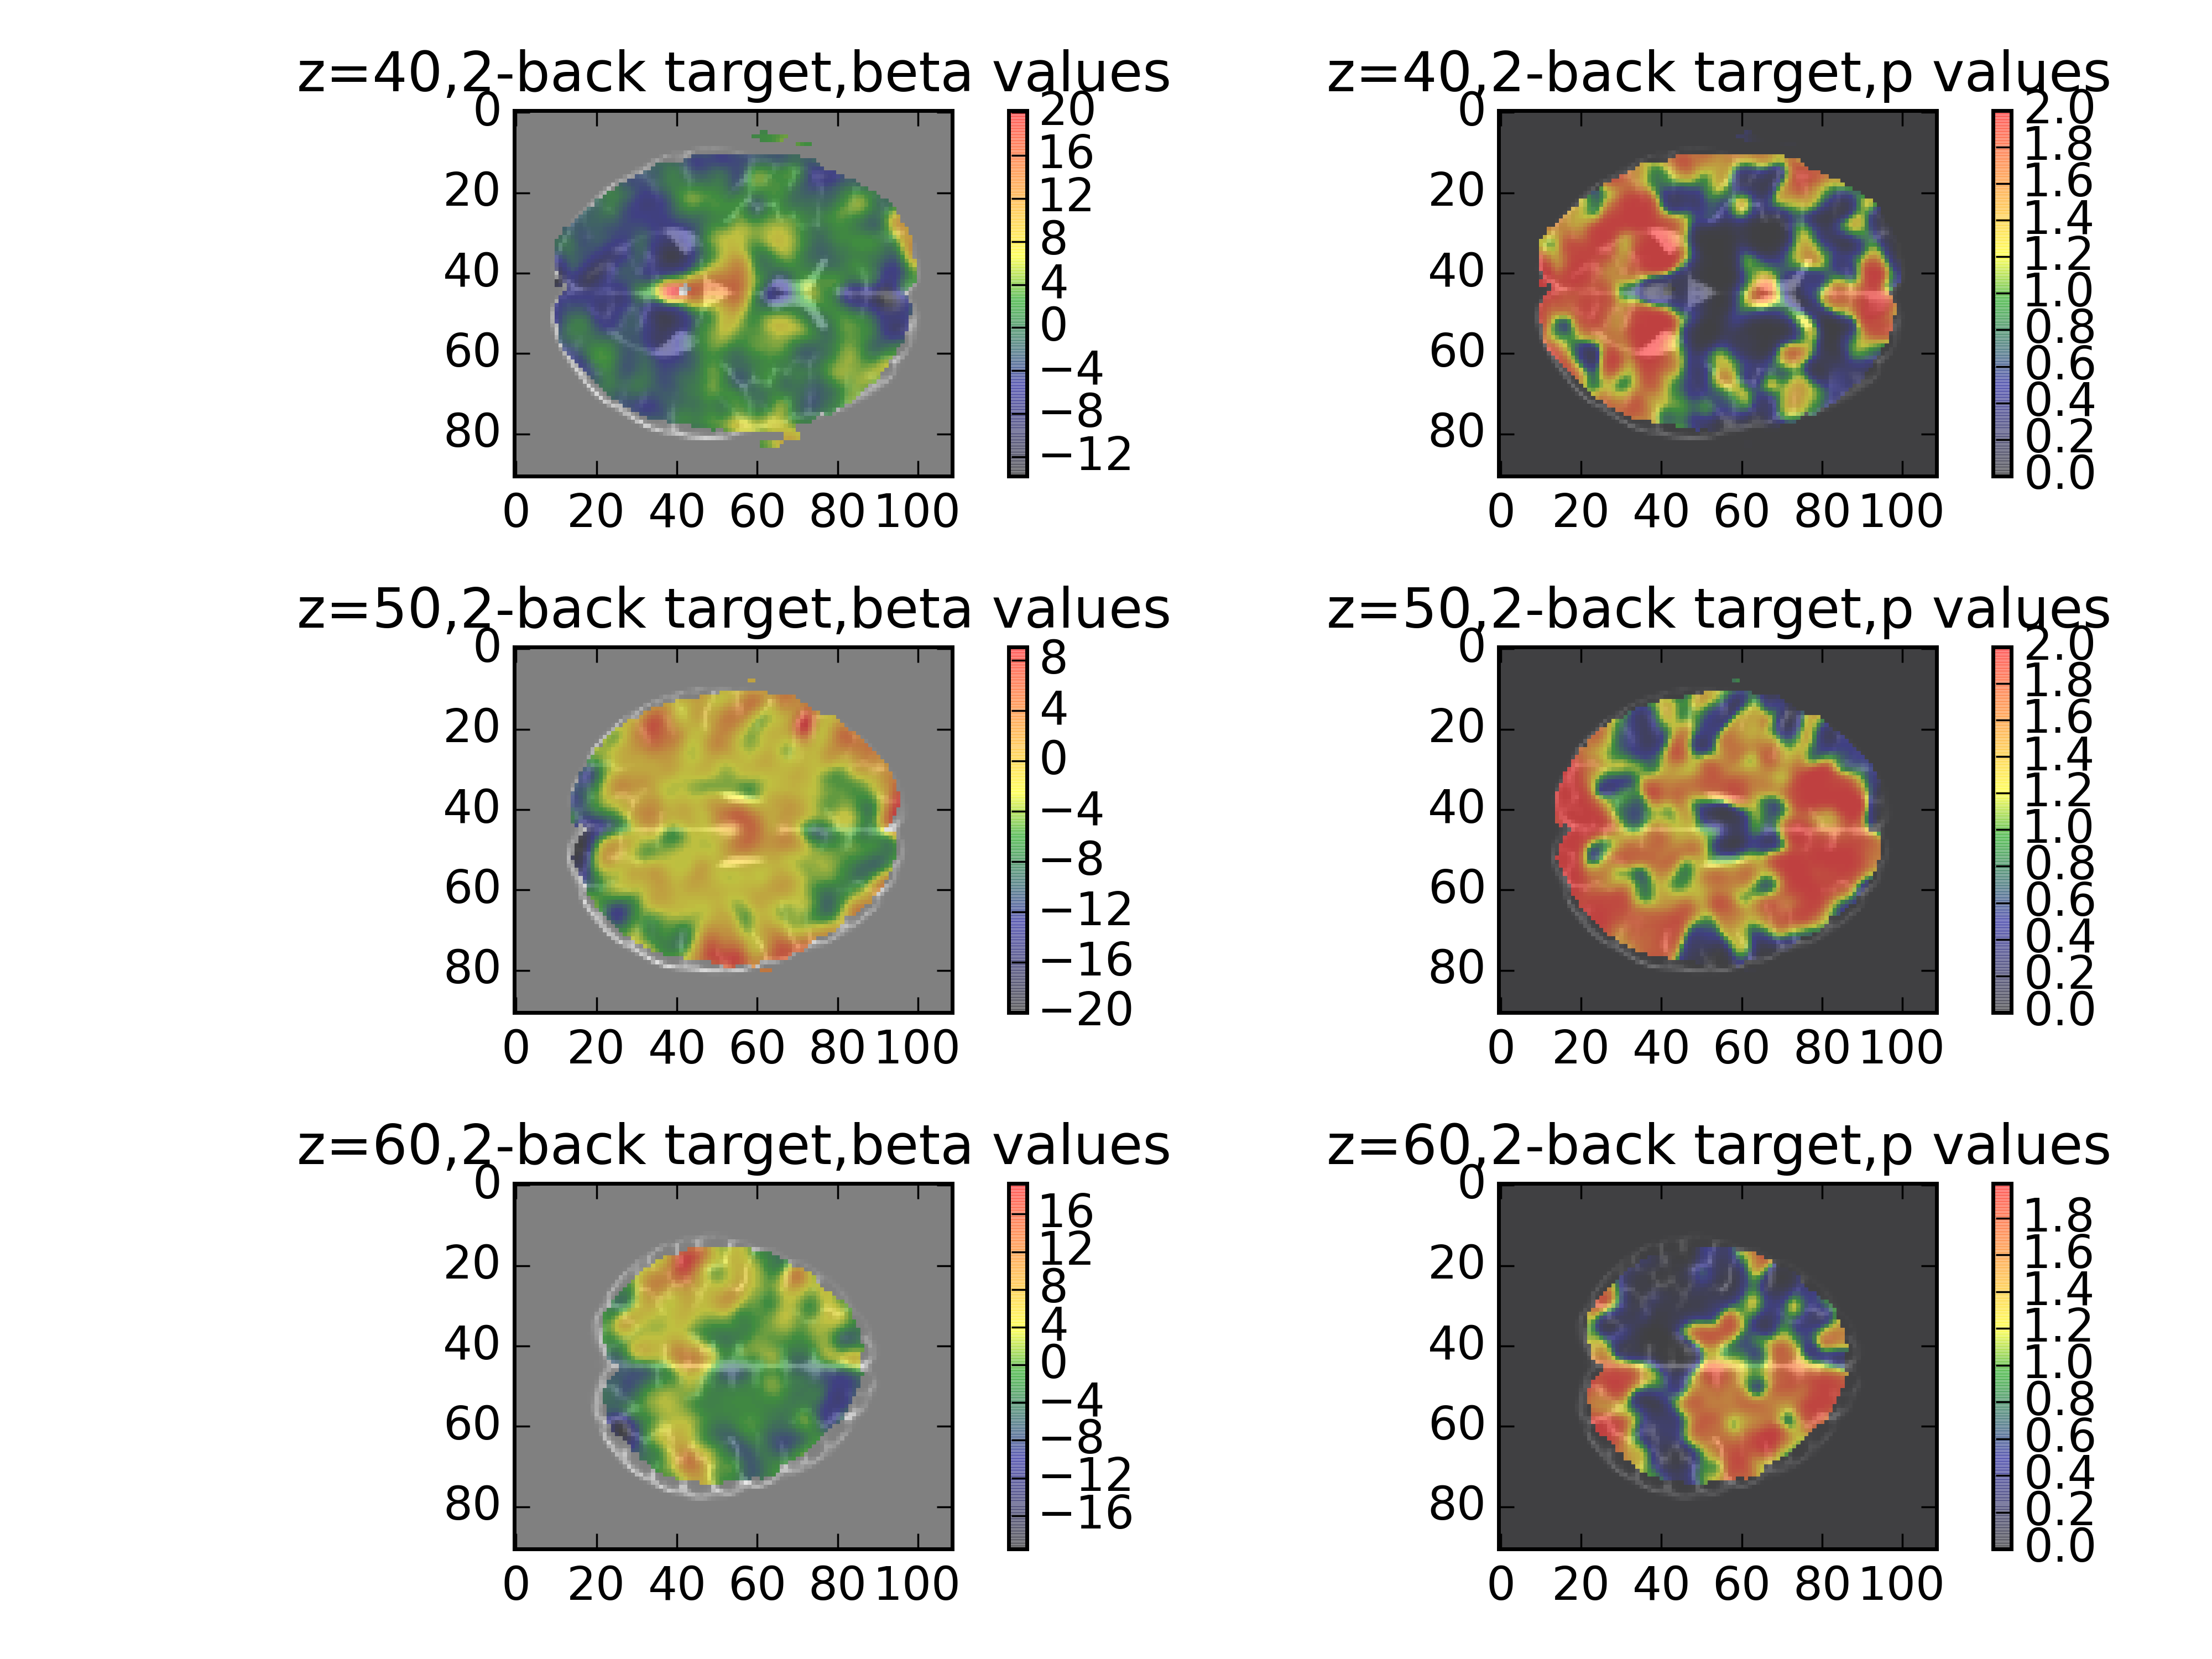
\includegraphics[scale=0.7]{figs/glm_graphs/sub011_target_betas_2_back.png}
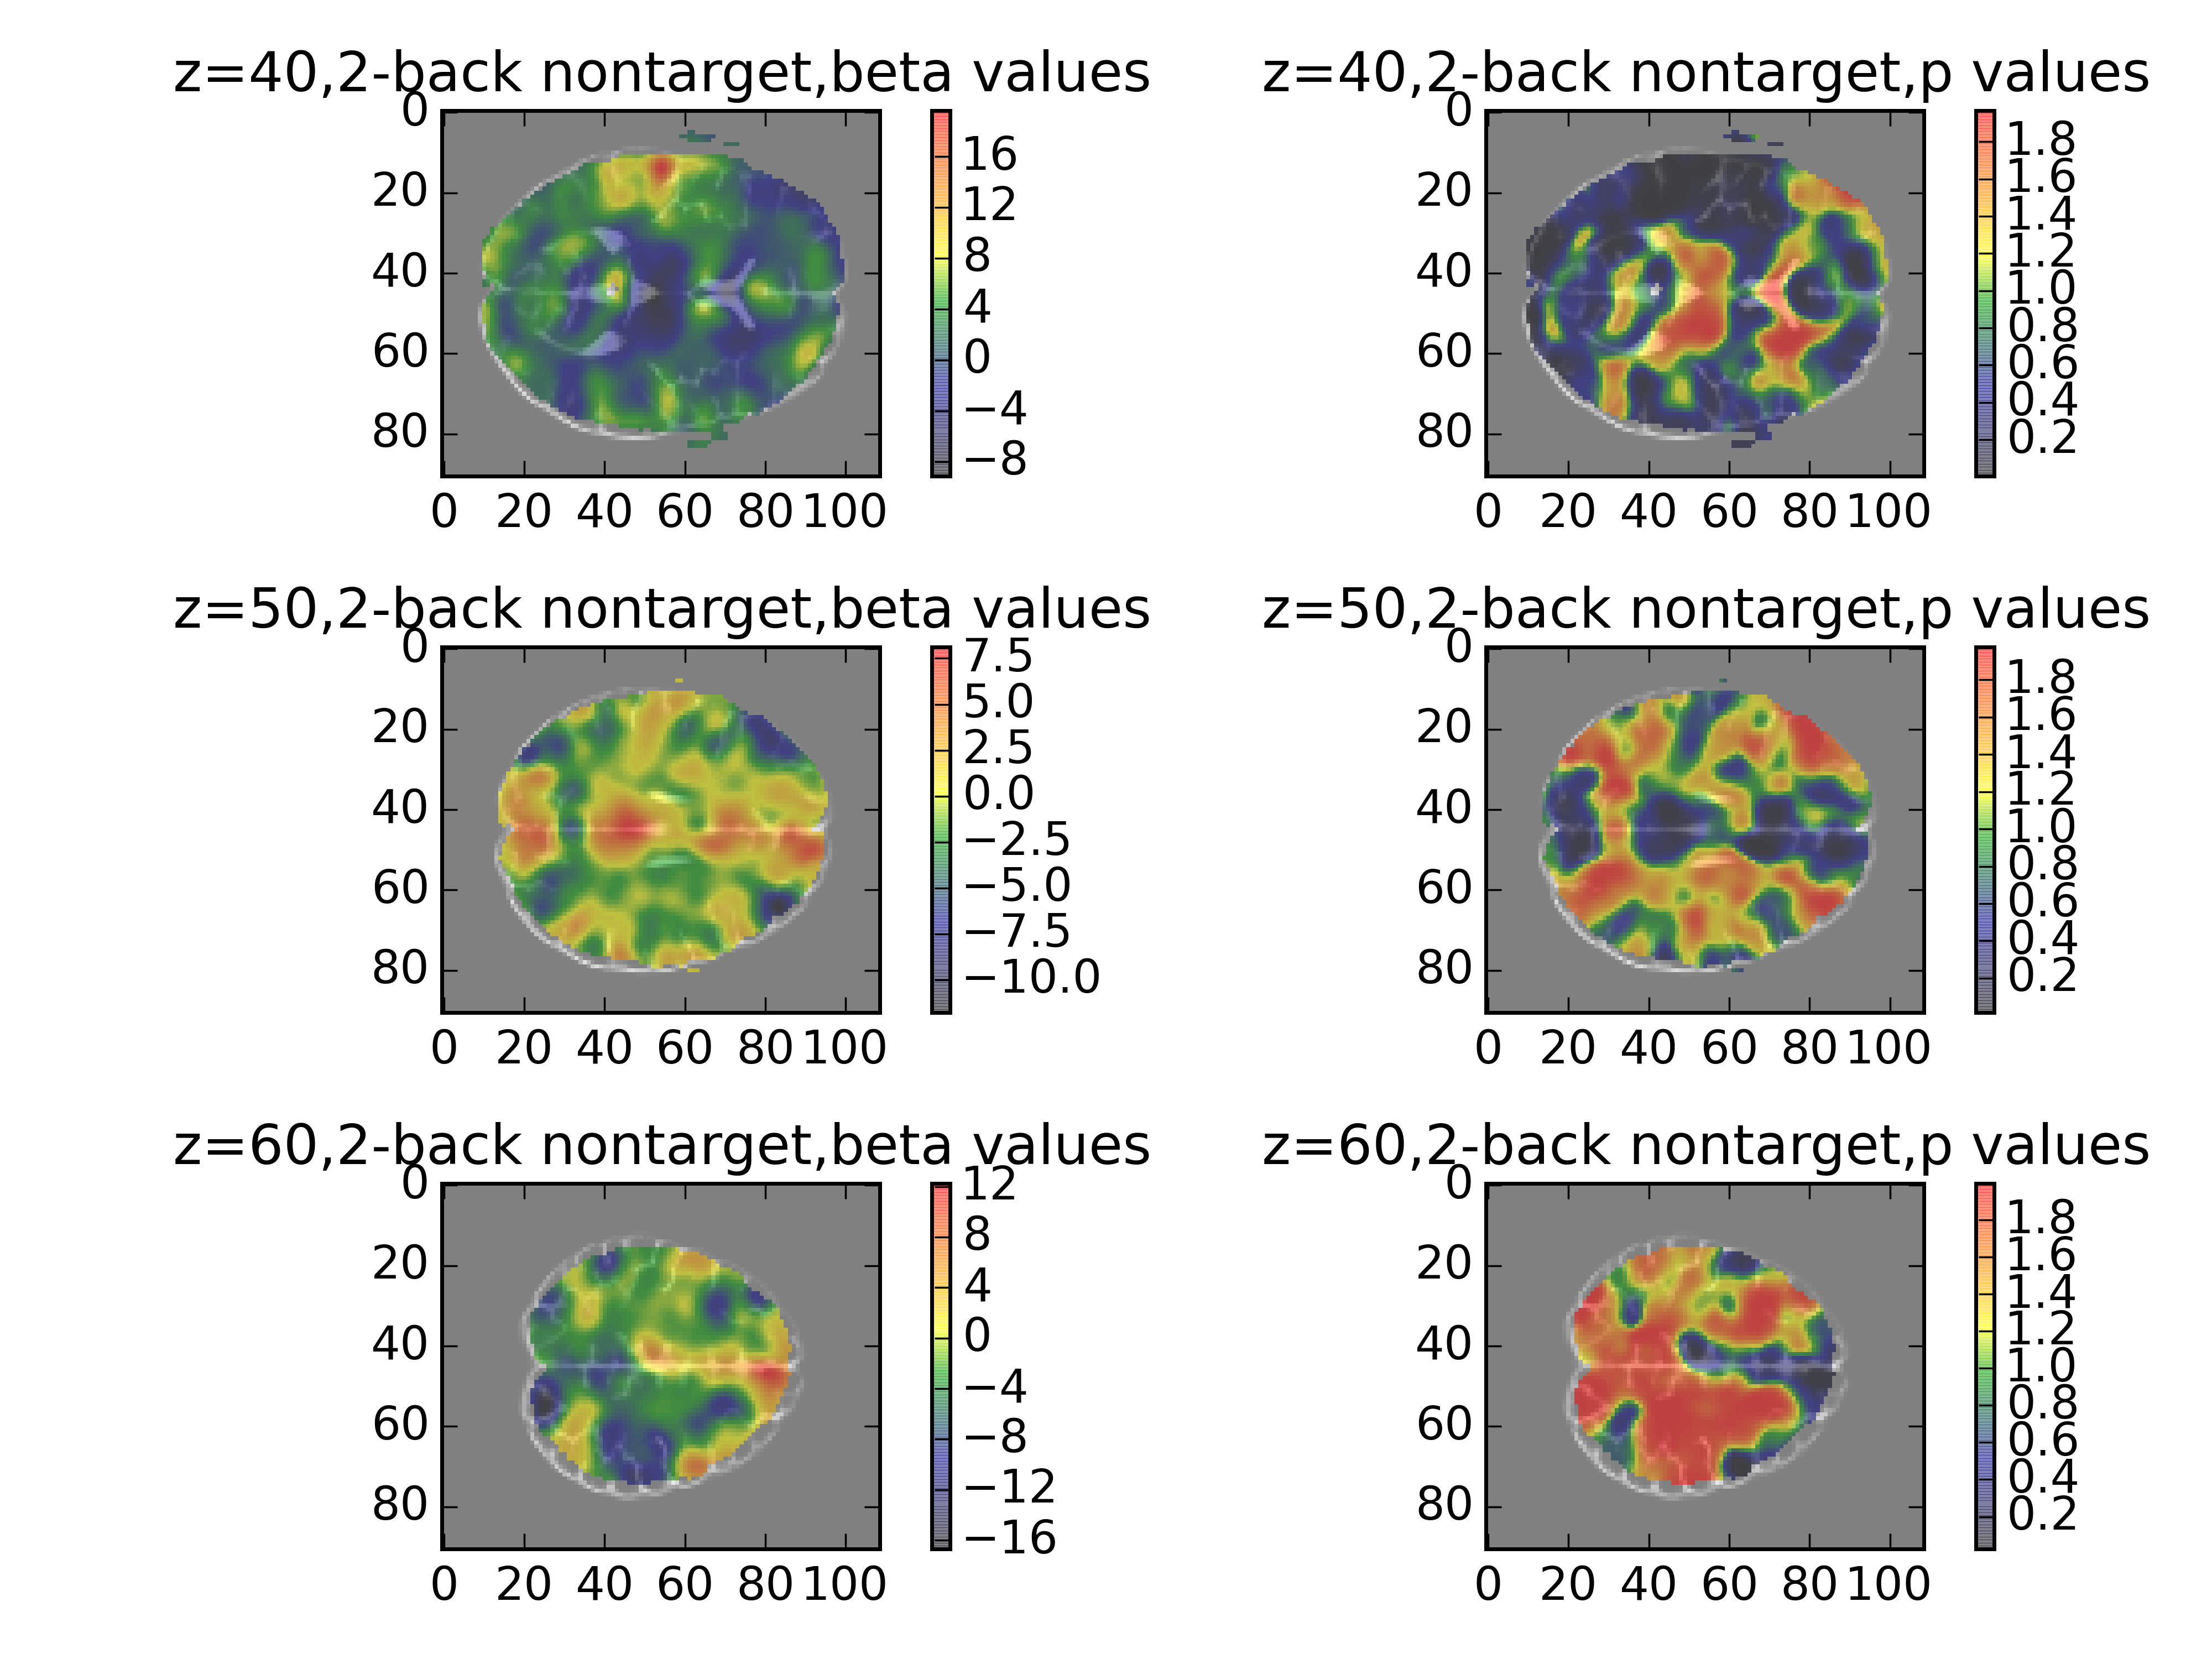
\includegraphics[scale=0.7]{figs/glm_graphs/sub011_nontarget_betas_2_back.png}
\caption{Above: 2-back target beta values and p values from two-tailed t tests against the null hypothesis of $\beta = 0$; Below: non-target beta values and p values from two-tailed t tests against the null hypothesis of $\beta = 0$}
\end{figure}

The two figures above display the observed activation patterns present in the 2-back task, which would be expected to activate regions of the prefrontal cortex more significantly than the 0-back task, on the basis that subjects must hold specific representations in memory in order to successfully complete this task. Furthermore, differences in the activation patterns between the target and nontarget 2-back tests shows that the activation during the target task is less distributed, activating more specific regions, as opposed to the generalized activity created by undergoing the nontarget 2-back task.

The nontarget 2-back task activation patterns and associated p-value maps for the coefficients estimated from the linear model indicate that the non-target task generates activity across many regions of the central nervous system, in particular subregions in the frontal lobes (as seen in slice z=60) as well as numerous occipital and midbrain region activations (as seen in the slices z=50 and z=40). The many regions activated in the nontarget 2-back analyses contrast sharply with the 2-back activations in the target group, as activations induced in the slices shown for that category are noticeably more focused in the occipital and frontal lobes.

The p-values associated with the coefficient estimates of the activation patterns in the 2-back target task show rather significant activation of frontal and midbrain regions, with these neural activations matching the more focused activation expected of a task more associated with inducing higher cognitive load. What is more, the differences in activation displayed by the two horizontal slices shown above illustrates how activation is distributed across the depths of the whole brain, in general activating frontal lobe regions associated with cognitive activity as well as occipital regions associated with visual task performance. With respect to the nontarget activation patterns displayed in the slices shown below, the map of p-values indicate that activation is much more generally distributed across the brain in the nontarget 2-back task, as would be expected of an error-based neural process.

\subsection{Connectivity Analysis}

\begin{figure}[H]
\centering
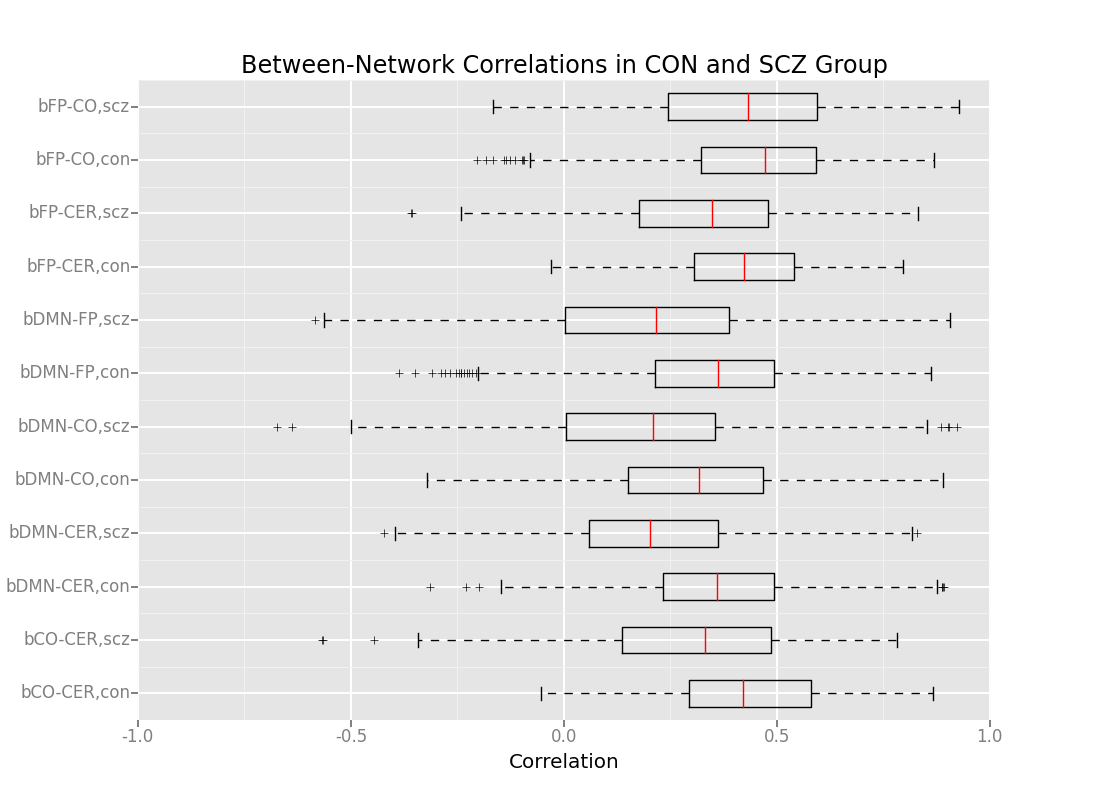
\includegraphics[scale=0.7]{figs/connectivity_plot.png}
\caption{The connectivity plot comparing schizophrenics (SCZ) and controls (CON) between networks}
\end{figure}

We performed the analysis on 20 subjects, including 12 SCZ (6 schizophrenias and 6 schizophrenia siblings) and 8 CON (4 controls and 4 control siblings). As shown in the figure above, the indivisuals with schizophrenia and their siblings (SCZ) showed an overall reduction in connecticity between the cognitive control networks as compared to CON as indicated in the boxplots of the correlations between networks for CON and SCZ. Previous studies concluded that there?s reduced distal connectivity for indivisuals with schizophrenia and especially between the FP and CER networks and the CO and CER networks (reference paper 1,2). However, the two results are not comparable in the following ways. 1) although we use a smaller dataset of 20 subjects versus 102 subjects used in the reference paper. 2) in the reference papers, many more nuisance regressors were removed from the BOLD time series. We only removed a few common noise regressors outlined in the method section. We obtained the similar result with the previous work and provided similar evidence that schizophrenia reflects a dysconnection syndrome.

Within-network correlations are not within the scope of our analysis. A graph showing the results for within-network correlations is included in the appendix.

\section{Discussion}

For now, we say that there is somewhat reduction in the response of the brain connectivity for the SCZ group compared to the CON, merely from the observation of the boxplots of the correlation r-values. In the future, we plan to perform permutation test to examine whether there?s any statistically significant difference of the correlations between the networks across the CON and SCZ group. Therefore, we can conclude whether there actually has a reduction in the connectivity for the SCZ with stronger evidence.

\bibliography{report}


\newpage
\appendix

\section{APPENDIX I - Results for Within-Network Correlations}

\begin{figure}[H]
\centering
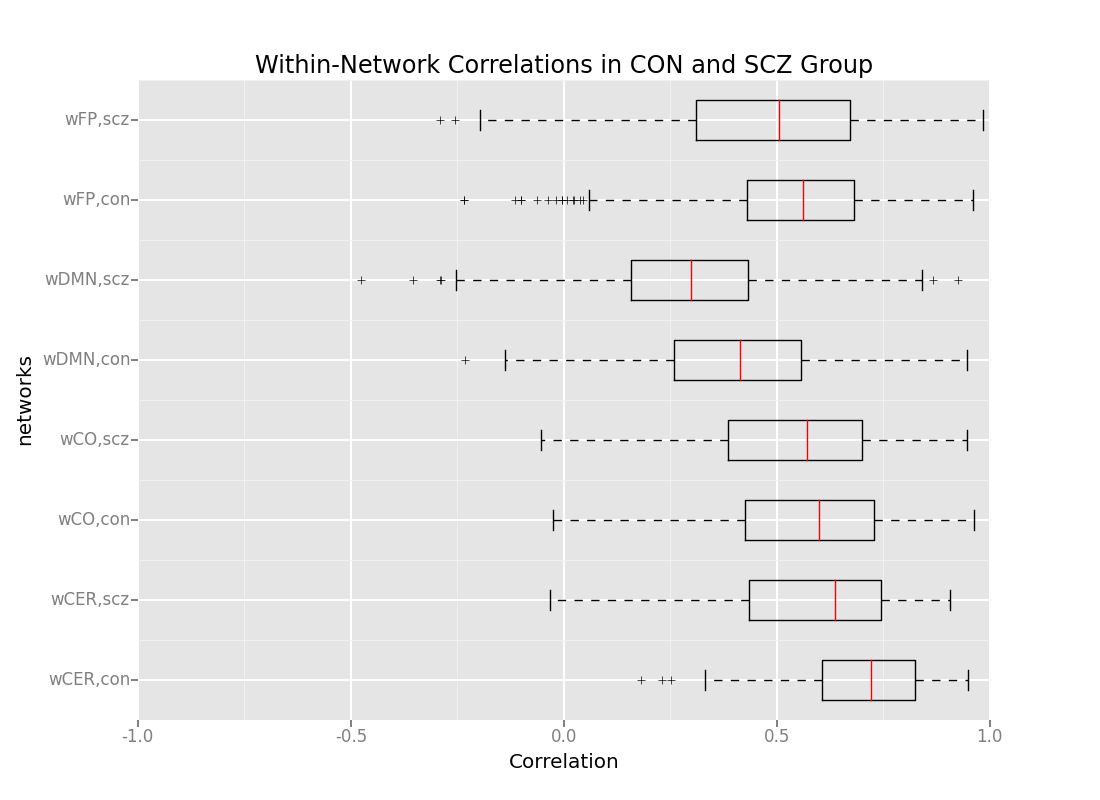
\includegraphics[scale=0.5]{figs/within_network_connectivity_plot.png}
\caption{The connectivity plot comparing schizophrenics (SCZ) and controls (CON) within networks}
\end{figure}

\section{APPENDIX II - Exploratory Analysis}

\subsection{Data Fetching and Preprocessing}

For all BOLD datasets, we removed the first five images to allow signals to
achieve steady state. In addition, we prepared scripts to detect the root mean
square (RMS) difference outliers using the inter-quartile range (IQR) to define
outliers. This was done because these images could contain a sudden widespread
shift in signals caused by hardware issues. We have run all the analysis with
the outliers removed so far, but will run a portion of the analysis with the
outliers in the future and discuss the impact of excluding outliers. 

Some preprocessing tasks are analysis-specific. As will be discussed in a later
section, we scaled BOLD signals per time step to use them as one of the feature
sets for k-means clustering. 

\subsection{Correlations with Baseline Functions}

This set of methods aim to produce an image identifying the regions which show
significant signal change in response to the task by calculating correlation
coefficients (r) between the bold signal along the time course and a reference
waveform, for each voxel. A high value of the correlation coefficient means that
fluctuation of the signal in the locale of the brain is task-dependent, hence
activated by the task.

For a bold signal X, and a reference waveform Y, the correlation coefficient is
calculated as bl
\begin{equation}
r = \frac{\Sigma_{i=1}^{n}  ( X-\bar{X}) ( Y-\bar{Y})}{\sqrt{ \Sigma_{i=1}^{n} (
    X-\bar{X} ) ^2 \Sigma_{i=1}^{n} ( Y-\bar{Y})  ^2 }}
\end{equation}

The two methods we are testing here are differentiated by two types of reference
waveforms: (1) square wave using on-off neural prediction from condition file
(SW method), and (2) a convolved function on neural predictions and a gamma
haemodynamic response function (HRF) (CF method). 

\begin{center}
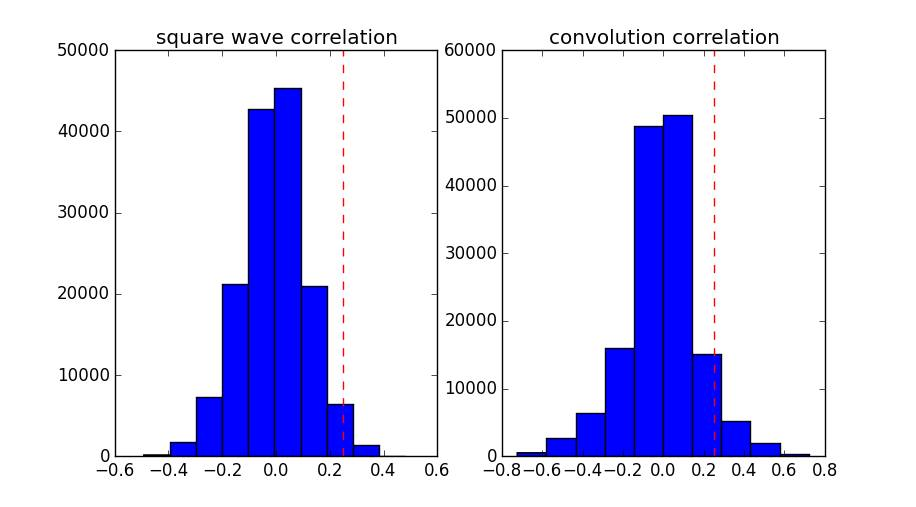
\includegraphics[width=16cm, height=8cm]{r_values_histogram.jpg}
\end{center}

Here, we want to compare the two types of analysis and decide on the better way
to find the activation regions. After calculating the correlations using both
square wave time course (SW method) and the convolved reference time course (CF
method), we plot the histogram of r-values to understand the range and
the distribution of the correlation. With that information, we decided on
the threshold 0.20 to say whether a voxel is active or not active. We plot the
voxels which correlate to the reference waveform with $r > 0.20$ in red, so that
we can visually examine the activation level of the voxels in the brain. By comparing
the activated regions under square wave time course (left) and convolved time
course (right), we can clearly see that it is hard for SW method to detect the
activation while the CR method gives more reasonable and detailed
results.Therefore, we will use the convolved reference waveform for detecting
the task-dependent voxels in our future analysis.

\begin{center}
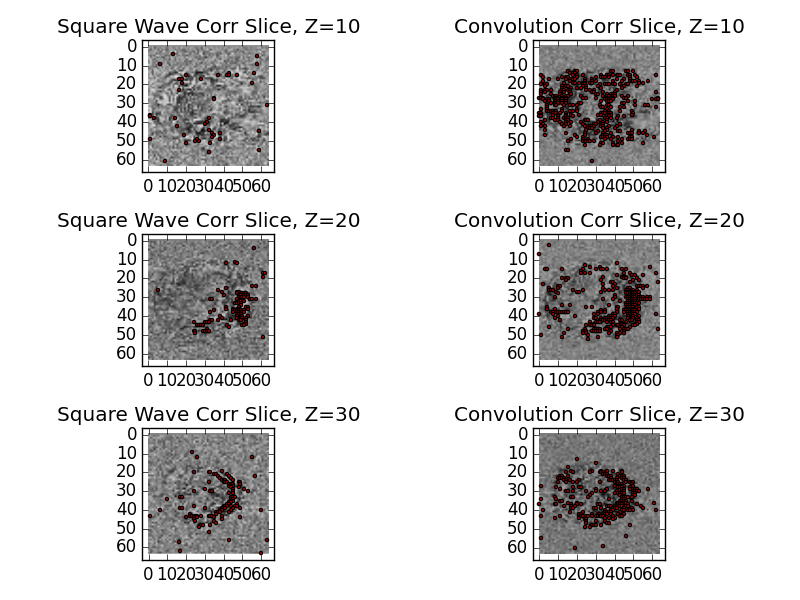
\includegraphics[width=12cm, height=12cm]{compare_correlations.png}
\end{center}

\subsection{Clustering with K-Means}

K-means clustering is an unsupervised technique which aims to partition n
observations into k clusters based on a feature set of n features. Each
observation is classified into the cluster with the nearest mean. In our case, n
is the number of voxels. k is chosen to be 5 although ideally, we should run
K-means with multiple k values \cite{venkataraman2009}. Clustering results
across the three runs of the same subject are merged together using a voting
algorithm \cite{dimitriadou2002}. We used three sets of features as described
below to obtain three sets of clustering results: (1) mean of BOLD signals over
time course for every voxel, (2) all signals in the time course for every voxel,
(3) all signals in the time course for every voxel, centered and normalized over
all signals in the corresponding time step. 

We do not involve the conditional file in the clustering. This is because the
underlying time courses are the same across methods as we compare across the
same subjects. Since Feature Set (1) only uses mean as a single feature, it
determines the clusters only based on intensity of the BOLD signals and can be
used a naive set of non-functional clusters (i.e. the other two or future
methods should deviate from this to reveal functional clusters). A comparison of
results across the three input feature sets is shown.

\begin{center}
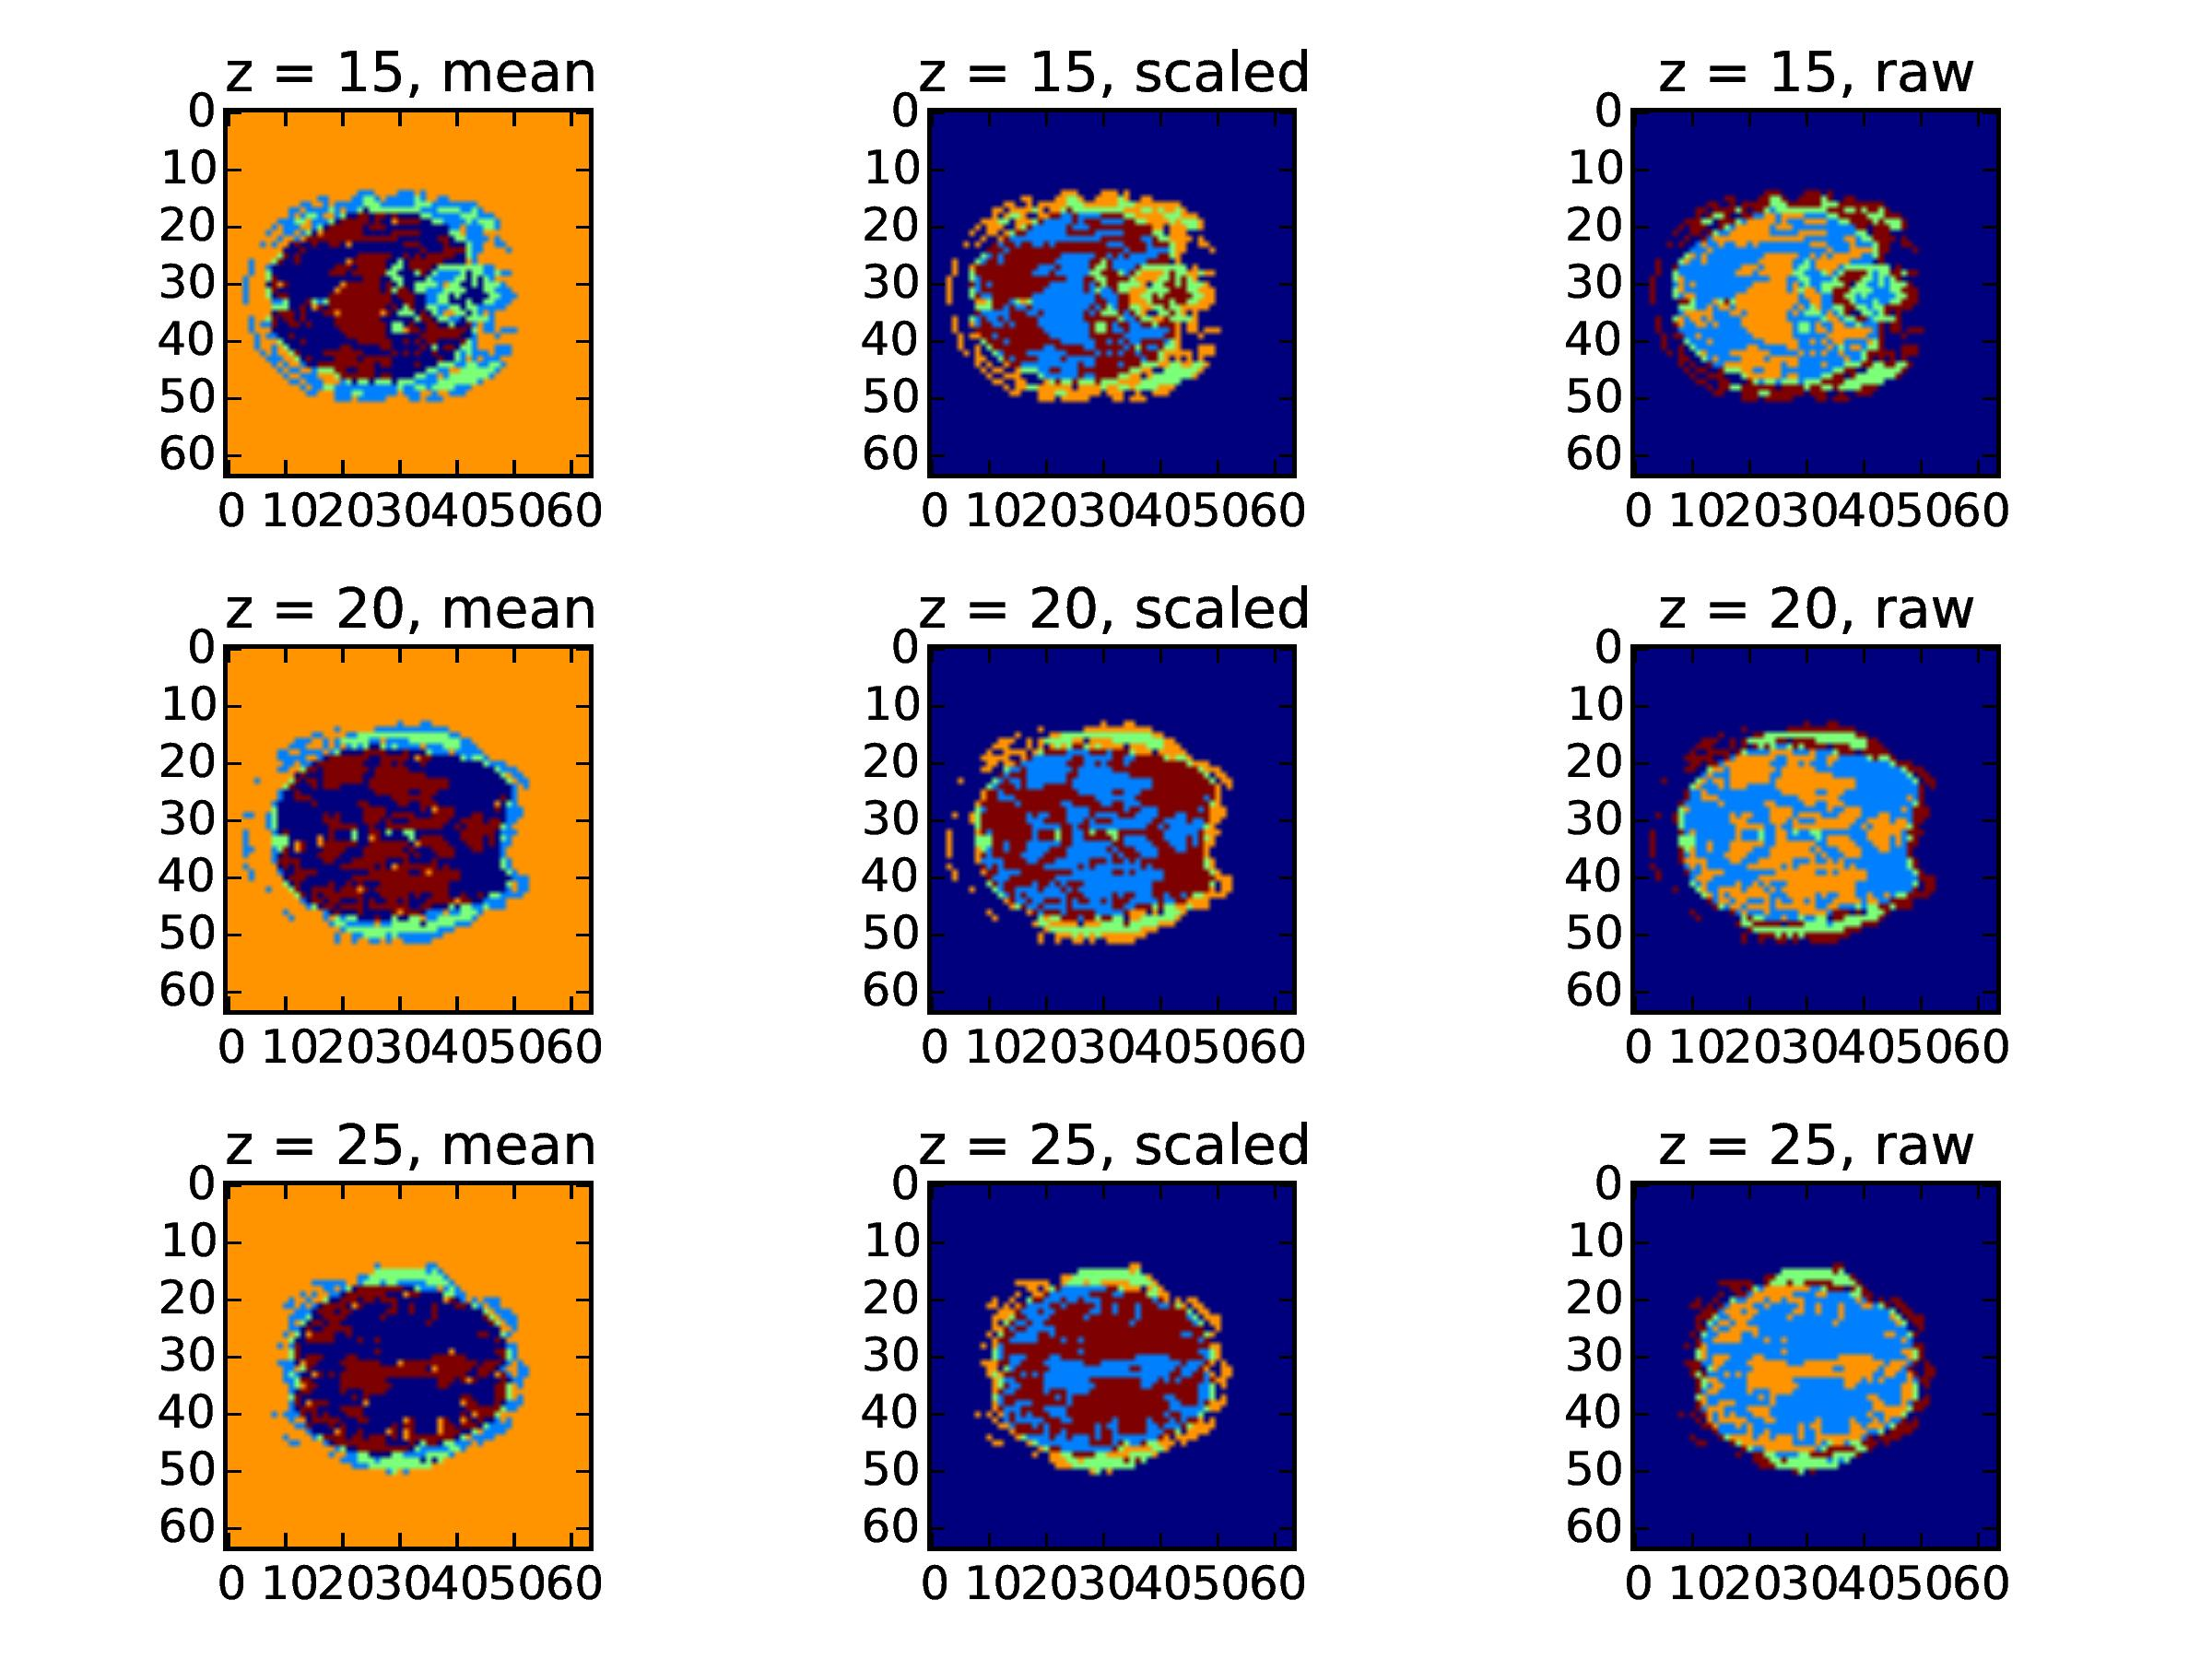
\includegraphics[width=12cm, height=12cm]{subject_across_methods.jpg}
\end{center}

Overall, basic and anatomical rather than functional clusters are revealed. For
example, the cerebral cortex is clustered together as well as the distinct
Thalamus-related region in the center of the brain.  Although there are visible
differences across subjects and runs, the differences across methods are almost
negligible. A scaled feature set has eliminated the intensity but does not
deviate from the naive clustering. The reason could be that there is too much
noise in the data. As an example, a drift term might be alone in determining the
clustering results. 

\subsection{Validation}

As we adopted a simple linear regression to fit our MRI data cross the predicted
neural time course, we need to check linear model assumptions before we conclude
validity of the model. One of the most important assumptions of linear model is
the normality of residuals.

Among the methods proposed to check normality, normal Q-Q plot is the most
commonly used. The Gaussian Q-Q plot compares residuals on the vertical axis
with a standard normal population on the horizontal axis. The linearity of the
points indicates normality. This method is straightforward and
intuitive. However, it has obvious weaknesses: (1) It can not evaluate multiple
vectors of residuals at same time; (2) there is no clear threshold to assert
normality. Therefore, it is not suitable for our normality test because we need
to check the normality on a per-voxel basis.

We used the Sharpiro-Wilk Test in which $H_0$ is $r_1,\dots ,r_n$ is normally
distributed. If the p-value we get from test statistic is less than the chosen
$\alpha$ level, then the null hypothesis is rejected and there is evidence that
the data tested are not from a normally distributed population.

Notice that we cannot naively compare all of these p-values individually with
$\alpha$, our type I error. Otherwise, our integrated type I error of test is
$\alpha^N$, vanishing as $N \rightarrow \infty$, which is too strict to check
multiple normality. Take the 11th subject as the example, if we just compare
p-values per voxel and $\alpha$ = 0.05, more than half of the test
($\frac{94397}{147456} =0.64$) will be rejected.

We have adopted several methods to handle this multiple comparison problem. 1)
Bonferroni procedure, in which reject the null if $p< \alpha/n$, where n is the
sample size. 2) Hochberg’s setup, in which order the p-values $p_1,\dots,p_n$ is
associate with corresponding hypothesis $H(1), \dots, H(n)$. Reject all
hypotheses $H(k) $ having $p(k)\leq \alpha/(n+1-k)$, where $ k=1,2,\dots,n$. 3)
Benjamini-Hochberg procedure, in which Order the p-values $P(1),P(2),\dots,P(n)$
and their associated hypothesis $H(1),\dots,H(n)$. Reject all hypotheses H(k)
having $P(k) \leq (k/n)\times \alpha $ ($k=1,\dots ,n$).

To be consistent with the previous example, these three methods are also
implemented on the fMRI data of 11th subject: (1) with Bonferroni correction and
outliers removed, there are 32896 voxels out of 147456 are not normally
distributed; (2) with Hochberg's procedure and outliers removed, there are 4843
voxels out of 147456 that are not normally distributed; (3) with
Benjamini-Hochberg's procedure and outliers removed, there are 0 voxels out of
147456 that are not normally distributed.

\section{APPENDIX III - Discussion of Exploratory Analyses}
\subsection{Exploratory Analyses}

\textbf{Extending and finetuning K-Means}: We will continue working towards our
goal of revealing functional clustering of the brain. This can be done by:
Improving the input features by inspecting and removing first principal
components of the datasets. This need to be done with care by visually
inspecting the principal components and consulting literature on the types and
characteristics of noise. One criterion of noise can be that the fluctuation has
a period clearly greater than the on-off cycle of the task. 

Improving input features by fitting the BOLD signals to a linear model and using
the residuals as input to K-means clustering. Using the same example above, a
drift term can be included in the design matrix so that it can be removed in the
residuals. This is the opposite of linear modelling to fit the data since in
this case, the aim is not to have a model to fit the data as best as possible
but to make use of the residuals in subsequent classification algorithms.

\begin{center}
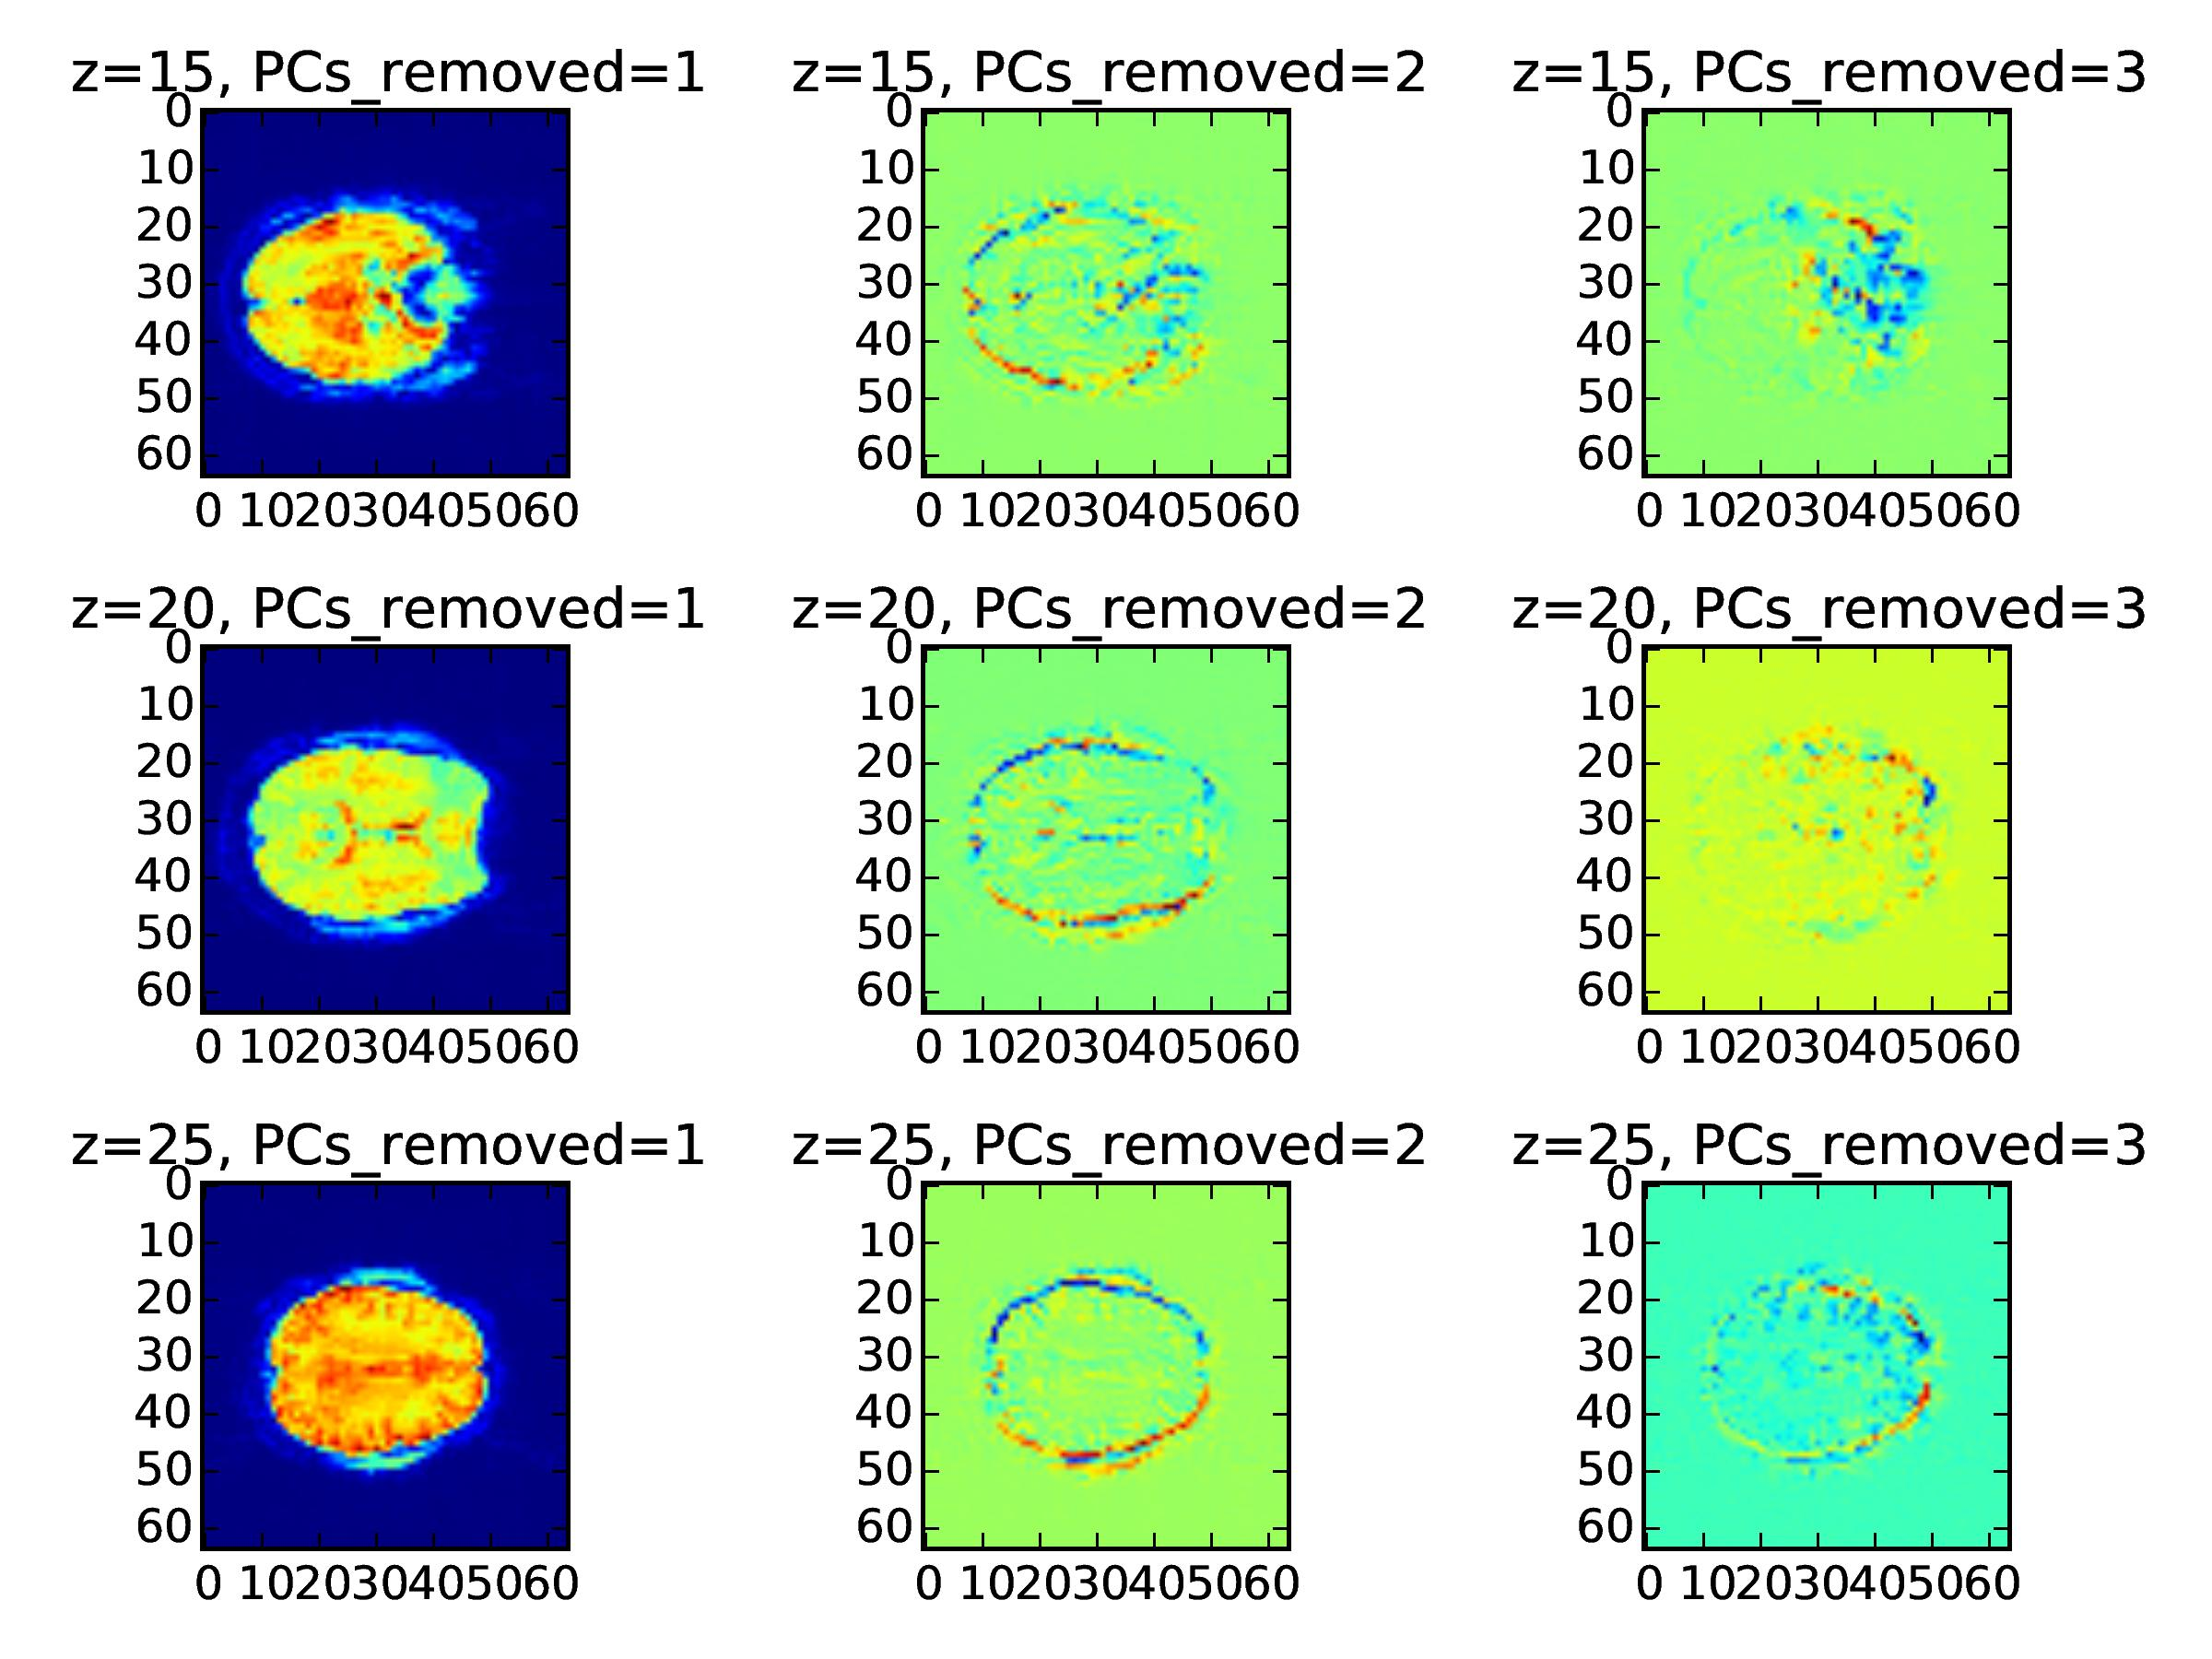
\includegraphics[width=12cm, height=12cm]{first_pcs_removed.jpg}
\end{center}

\textbf{Improving other analyses}: applying the same methods of noise reduction in
K-means in other analyses, 
such as correlations to refine the results and possibly make comparisons with
K-means. This is because both types of analysis serve to discover activation
regions. 

\textbf{Scaling analyses to make comparisons across different subject groups}: at this
stage, we focused on developing the scripts to analyze and make comparisons
within single subjects. From now on, we will apply the analyses across subject
groups in order to draw conclusions on differences in healthy and schizophrenia
subjects. To achieve this, some averaging techniques are necessary for
cross-group comparison. One example already mentioned is the merging algorithm
for K-means clustering. 

\textbf{Research other machine learning techniques to further
explore activation regions}: a greater variety of methods will allow us to reveal different insights about the data and make comparisons richer, giving us the freedom to explore and discuss the merits of different machine learning algorithms with respect to fMRI. 

\textbf{Talairach Space Transformation}: since one of our goals is to demonstrate activation regions revealed by the
datasets and compare those provided in the literature, we need to transform
coordinates to and back from Talairach space since most coordinates in
literature are provided in that space.

\subsection{Lessons Learned}

The dataset we use for our analysis is multi-layered and ambiguous in some sense. In our dataset, there are 3 runs for each subject as well as 7 condition files explaining the scan timeline for each run. In our analysis, the condition record we used has fractional seconds for scan duration (0.769951s), a very small proportion of the TR. In the example analysis seen in class, the durations we dealt with were always a multiple of the TR (2.5s). In this case, if we use the same TR as the scale, we would have to divide 0.769951 by 2.5 (around 0.30798) to fit the scale, the resulting convolution will deviate from the real scenario, causing bias. Therefore, we adopted the following strategy to tackle this problem: (1) rescaling data, converting from 2.5s to 0.1s as the unit; (2) in each 2.5s interval, choosing the median value to represent convolved data in that time interval; (3) convolving the data using the standard approach. This generates the convolved function we used in the analysis of correlations. 

Furthermore, the analysis done in the paper by Repovs \textit{et al.}�� is based on the Resting State dataset, in which they investigate the connectivity of the regions in the brain for patients and healthy controls \cite{repovs2012}. We tried to reproduce their result using the data; however, we encountered the problem of separating the resting state data from the rest of the BOLD signals. Consequently, it is important for us to find another potential, executable topic given the current dataset and develop a coherent rigorous statistical analysis.


\end{document}
